% 注意事项:编译两次,以确保目录、页码完整显示

\def\allfiles{}

\documentclass[14pt,a4paper,UTF8,twoside]{article}

% Formatting Packages ——————————————————————————————————————
\usepackage{multicol}
\usepackage{multirow}
\usepackage{enumitem}
\usepackage{indentfirst}
\usepackage[toc]{multitoc}

% Math & Physics Packages ————————————————————————————
\usepackage{amsmath, amsthm, amsfonts, amssymb}
\usepackage{setspace}
\usepackage{physics}
\usepackage{cancel}
\usepackage{nicefrac}
\usepackage{unicode-math} % 允许数学公式使用特定字体

% Image-related Packages —————————————————————————————
\usepackage{float} % 浮动体环境
\usepackage{subcaption} % 子图包
\usepackage{graphics, graphicx}
\usepackage{tikz, tikz-qtree}
\usepackage{mdframed}
\usepackage{lmodern}
\usetikzlibrary{arrows.meta}
\usetikzlibrary{shapes.geometric, arrows}
\tikzstyle{startstop} = [rectangle, rounded corners, minimum width=3cm, minimum height=1cm,text centered, draw=black, fill=red!30]
\tikzstyle{process} = [rectangle, minimum width=3cm, minimum height=1cm, text centered, draw=black, fill=blue!30]
\tikzstyle{arrow} = [thick,->,>=stealth]

\usepackage{pgfplots}
\pgfplotsset{compat=1.18}
\usepackage{xcolor}
\usepackage{fourier-orns}
\usepackage{lipsum}

% Colour Palette ——————————————————————————————————————
\definecolor{merah}{HTML}{F4564E}
\definecolor{merahtua}{HTML}{89313E}
\definecolor{biru}{HTML}{60BBE5}
\definecolor{birutua}{HTML}{412F66}
\definecolor{hijau}{HTML}{59CC78}
\definecolor{hijautua}{HTML}{366D5B}
\definecolor{kuning}{HTML}{FFD56B}
\definecolor{jingga}{HTML}{FBA15F}
\definecolor{ungu}{HTML}{8C5FBF}
\definecolor{lavender}{HTML}{CBA5E8}
\definecolor{merjamb}{HTML}{FFB6E0}
\definecolor{mygray}{HTML}{E6E6E6}
\definecolor{mygreen}{rgb}{0,0.6,0}
\definecolor{mymauve}{rgb}{0.58,0,0.82}

% Theorems ————————————————————————————————————————————
\usepackage{tcolorbox}
\usepackage{changepage}
\tcbuselibrary{skins,breakable,theorems}

\newcounter{hitung}
\setcounter{hitung}{\thesection}

\makeatletter
	% Proof 证明如下
	\def\tcb@theo@widetitle#1#2#3{\hbox to \textwidth{\textsc{\large#1}\normalsize\space#3\hfil(#2)}}
	\tcbset{
		theorem style/theorem wide name and number/.code={ \let\tcb@theo@title=\tcb@theo@widetitle},
		proofbox/.style={skin=enhancedmiddle,breakable,parbox=false,boxrule=0mm,
			check odd page, toggle left and right, colframe=black!20!white!92!hijau,
			leftrule=8pt, rightrule=0mm, boxsep=0mm,arc=0mm, outer arc=0mm,
			left=3mm,right=3mm,top=0mm,bottom=0mm, toptitle=0mm,
			bottomtitle=0mm,colback=gray!3!white!98!biru, before skip=8pt, after skip=8pt,
			before={\par\vskip-2pt},after={\par\smallbreak},
		},
	}
	\newtcolorbox{ProofBox}{proofbox}
	\makeatother
	
	\let\realproof\proof
	\let\realendproof\endproof
	\renewenvironment{proof}[1][Prove:]{\ProofBox\strut\textsc{#1}\space}{\endProofBox}
        \AtEndEnvironment{proof}{\null\hfill$\blacksquare$}
        % Definition 定义环境
	\newtcbtheorem[use counter=hitung, number within=section]{dfn}{定义}
	{theorem style=theorem wide name and number,breakable,enhanced,arc=3.5mm,outer arc=3.5mm,
		boxrule=0pt,toprule=1pt,leftrule=0pt,bottomrule=1pt, rightrule=0pt,left=0.2cm,right=0.2cm,
		titlerule=0.5em,toptitle=0.1cm,bottomtitle=-0.1cm,top=0.2cm,
		colframe=white!10!biru,
		colback=white!90!biru,
		coltitle=white,
		shadow={1.3mm}{-1.3mm}{0mm}{gray!50!white}, % 添加阴影
        coltext=birutua!60!gray, title style={white!10!biru}, rbefoe skip=8pt, after skip=8pt,
		fonttitle=\bfseries,fontupper=\normalsize}{dfn}

	% 答题卡
	\newtcbtheorem[use counter=hitung, number within=section]{ans}{解答}
	{theorem style=theorem wide name and number,breakable,enhanced,arc=3.5mm,outer arc=3.5mm,
		boxrule=0pt,toprule=1pt,leftrule=0pt,bottomrule=1pt, rightrule=0pt,left=0.2cm,right=0.2cm,
		titlerule=0.5em,toptitle=0.1cm,bottomtitle=-0.1cm,top=0.2cm,
		colframe=white!10!biru,
		colback=white!90!biru,
		coltitle=white,
		shadow={1.3mm}{-1.3mm}{0mm}{gray!50!white}, % 添加阴影
        coltext=birutua!60!gray, title style={white!10!biru}, before skip=8pt, after skip=8pt,
		fonttitle=\bfseries,fontupper=\normalsize}{ans}

	% Axiom
	\newtcbtheorem[use counter=hitung, number within=section]{axm}{公理}
	{theorem style=theorem wide name and number,breakable,enhanced,arc=3.5mm,outer arc=3.5mm,
		boxrule=0pt,toprule=1pt,leftrule=0pt,bottomrule=1pt, rightrule=0pt,left=0.2cm,right=0.2cm,
		titlerule=0.5em,toptitle=0.1cm,bottomtitle=-0.1cm,top=0.2cm,
		colframe=white!10!biru,colback=white!90!biru,coltitle=white,
		shadow={1.3mm}{-1.3mm}{0mm}{gray!50!white!90}, % 添加阴影
        coltext=birutua!60!gray,title style={white!10!biru},before skip=8pt, after skip=8pt,
		fonttitle=\bfseries,fontupper=\normalsize}{axm}
 
	% Theorem
	\newtcbtheorem[use counter=hitung, number within=section]{thm}{定理}
	{theorem style=theorem wide name and number,breakable,enhanced,arc=3.5mm,outer arc=3.5mm,
		boxrule=0pt,toprule=1pt,leftrule=0pt,bottomrule=1pt, rightrule=0pt,left=0.2cm,right=0.2cm,
		titlerule=0.5em,toptitle=0.1cm,bottomtitle=-0.1cm,top=0.2cm,
		colframe=white!10!merah,colback=white!75!pink,coltitle=white, coltext=merahtua!80!merah,
		shadow={1.3mm}{-1.3mm}{0mm}{gray!50!white!90}, % 添加阴影
		title style={white!10!merah}, before skip=8pt, after skip=8pt,
		fonttitle=\bfseries,fontupper=\normalsize}{thm}
	
	% Proposition
	\newtcbtheorem[use counter=hitung, number within=section]{prp}{命题}
	{theorem style=theorem wide name and number,breakable,enhanced,arc=3.5mm,outer arc=3.5mm,
		boxrule=0pt,toprule=1pt,leftrule=0pt,bottomrule=1pt, rightrule=0pt,left=0.2cm,right=0.2cm,
		titlerule=0.5em,toptitle=0.1cm,bottomtitle=-0.1cm,top=0.2cm,
		colframe=white!10!hijau,colback=white!90!hijau,coltitle=white, coltext=hijautua!80!brown,
		shadow={1.3mm}{-1.3mm}{0mm}{gray!50!white}, % 添加阴影
		title style={white!10!hijau}, before skip=8pt, after skip=8pt,
		fonttitle=\bfseries,fontupper=\normalsize}{prp}


	% Example
	\newtcolorbox[use counter=hitung, number within=section]{cth}[1][]{breakable,
		colframe=white!10!jingga, coltitle=white!90!jingga, colback=white!85!jingga, coltext=black!10!brown!50!jingga, colbacktitle=white!10!jingga, enhanced, fonttitle=\bfseries,fontupper=\normalsize, attach boxed title to top left={yshift=-2mm}, before skip=8pt, after skip=8pt,
		title=Itemize~\thetcbcounter \ \ #1}

	% Catatan/Note
	\newtcolorbox{ctt}[1][]{enhanced, 
		left=4.1mm, borderline west={8pt}{0pt}{white!10!kuning}, 
		before skip=6pt, after skip=6pt, 
		colback=white!85!kuning, colframe= white!85!kuning, coltitle=orange!60!kuning!25!brown, coltext=orange!60!kuning!25!brown,
		fonttitle=\bfseries,fontupper=\normalsize, before skip=8pt, after skip=8pt,
		title=\underline{Notice}  #1}
	
	% Komentar/Remark
	\newtcolorbox{rmr}[1][]{
		,arc=0mm,outer arc=0mm,
		boxrule=0pt,toprule=1pt,leftrule=0pt,bottomrule=5pt, rightrule=0pt,left=0.2cm,right=0.2cm,
		titlerule=0.5em,toptitle=0.1cm,bottomtitle=-0.1cm,top=0.2cm,
		colframe=white!10!kuning,colback=white!85!kuning,coltitle=white, coltext=orange!60!kuning,
		fonttitle=\bfseries,fontupper=\normalsize, before skip=8pt, after skip=8pt,
		title=Question  #1}

\usepackage{booktabs} % 表格库
\usepackage{titlesec} % 标题库
\usepackage{fancyhdr} % 页眉页脚库
\usepackage[sorting=none]{biblatex}
\usepackage{array}
\usepackage{longtable}
\usetikzlibrary{positioning, arrows.meta}
\addbibresource{references.bib} % 指定你的.bib文件名称

\date{} % 留空,以让编译时去除日期

%———————————————注意事项—————————————————%

% 1、如果编译显示失败,但没有错误信息,就是 filename.pdf 正在被占用
% 2、在文件夹中的终端使用 Windows > xelatex filename.tex 也可编译

%—————————————华东师范大学———————————————%

% 论文制作时须加页眉,页眉从中文摘要开始至论文末
% 偶数页码内容为:华东师范大学硕士学位论文,奇数页码内容为学位论文题目

%————————定义 \section 的标题样式————————%

% 注意:\chapter 等命令,内部使用的是 \thispagestyle{plain} 的排版格式
% 若需要自己加上页眉,实际是在用 \thispagestyle{fancy} 的排版格式
% 加上下面这一段指令,就能够让 \section 也使用 fancy 的排版格式
% 本质就是让目录、第一页也能够显示页眉、页脚

\fancypagestyle{plain}{
  \pagestyle{fancy}
}

\title{华东师范大学软件学院实验报告} % 模板
\titleformat{\section}
    {\normalfont\bfseries\Large} % 字体大小、字体系列(\bfseries 为加粗)
    {\thesection}{1em}{}

% ———————————设置章节的中文格式———————————%
\renewcommand\thesection{\chinese{section} \hspace{0pt}}
\renewcommand\thesubsection{\arabic{subsection} \hspace{0pt}}
% \renewcommand\thesubsubsection{\alph{subsubsection} \hspace{0pt}} % 字母编号
% \hspace{0pt} 是为了确保在章节编号和章节题目之间不要有空格,使得排版更为美观
    
%—————————————页面基础设置———————————————%

\usepackage{geometry}
\geometry{left=10mm, right=10mm, top=20mm, bottom=20mm}

%————————————设置页眉、页脚——————————————%

\pagestyle{fancy} % 设置 plain style 的属性

% 设置页眉

\fancyhead[RE]{\footnotesize \leftmark} % Right Even 偶数页右侧显示章名 \leftmark 最高级别章名
\fancyhead[LO]{\footnotesize \rightmark} % Left Odd 奇数页左侧显示节名 \rightmark 第二级别节名
\fancyhead[C]{华东师范大学软件学院实验报告} % Center 居中显示
\fancyhead[LE,RO]{~\thepage~} % 在偶数页的左侧,奇数页的右侧显示页码
\renewcommand{\headrulewidth}{1.2pt} % 页眉与正文之间的水平线粗细

% 设置页脚:在每页的右下脚以斜体显示书名

\fancyfoot[RO,RE]{\it Lab Report By \LaTeX} % 使用意大利斜体显示
\renewcommand{\footrulewidth}{0.5pt} % 页脚水平线宽度

%——————设置页码:在底部居中显示页码———————%

\usepackage{lastpage} % 页码数库
\pagestyle{fancy}
\fancyfoot[C]{\kaishu 第 \thepage 页 \ 共 \pageref{LastPage} 页} % LastPage 需要二次编译以获取总页数

%——————————————代码块设置———————————————%

\usepackage{listings} % 代码块包
\lstset {
    backgroundcolor=\color{white},   % choose the background color; you must add \usepackage{color} or \usepackage{xcolor}
    basicstyle=\footnotesize,        % the size of the fonts that are used for the code
    breakatwhitespace=false,         % sets if automatic breaks should only happen at whitespace
    breaklines=true,                 % sets automatic line breaking
    captionpos=bl,                   % sets the caption-position to bottom
    commentstyle=\color{mygreen},    % comment style
    deletekeywords={...},            % if you want to delete keywords from the given language
    escapeinside={\%*}{*},           % if you want to add LaTeX within your code
    extendedchars=true,              % lets you use non-ASCII characters; for 8-bits encodings only, does not work with UTF-8
    frame=single,                    % adds a frame around the code
    keepspaces=true,                 % keeps spaces in text, useful for keeping indentation of code (possibly needs columns=flexible)
    keywordstyle=\color{blue},       % keyword style
    % language=Python,               % the language of the code
    morekeywords={*,...},            % if you want to add more keywords to the set
    numbers=left,                    % where to put the line-numbers; possible values are (none, left, right)
    numbersep=5pt,                   % how far the line-numbers are from the code
    numberstyle=\tiny\color{mygray}, % the style that is used for the line-numbers
    rulecolor=\color{black},         % if not set, the frame-color may be changed on line-breaks within not-black text (e.g. comments (green here))
    showspaces=false,                % show spaces everywhere adding particular underscores; it overrides 'showstringspaces'
    showstringspaces=false,          % underline spaces within strings only
    showtabs=false,                  % show tabs within strings adding particular underscores
    stepnumber=1,                    % the step between two line-numbers. If it's 1, each line will be numbered
    stringstyle=\color{orange},      % string literal style
    tabsize=2,                       % sets default tabsize to 2 spaces
    % title=Python Code              % show the filename of files included with \lstinputlisting; also try caption instead of title
}

% 注释掉的部分用于后续插入代码,参数可调整,格式如下:

% 1、直接插入
% \begin{lstlisting}[language = ? , title = { ? } ]
%       Your code here.
% \end{lstlisting}

% 2、文件插入
% \lstinputlisting[language = C , title = ?.c] {filename.c}

%———————————————字体设置————————————————%

\usepackage{fontspec} % 允许设置字体
\usepackage[utf8]{inputenc}
\usepackage{ctex}
\usepackage{pifont}
\linespread{1.2}
% \setCJKmainfont{SimSun} % 设置正文罗马族的 CJK 字体
\renewcommand{\texttt}[1]{\textcolor{blue}{\ttfamily #1}}

%———————————————超链接设置——————————————%

\usepackage[hidelinks]{hyperref}
\hypersetup{
    pdfstartview=FitH, % 设置PDF文档打开时的初始视图为页面宽度适应窗口宽度(即页面水平适应)
    CJKbookmarks=true, % 用对CJK(中文、日文、韩文)字符的书签支持,确保这些字符在书签中正确显示
    bookmarksnumbered=true, % 书签带有章节编号。这对有章节编号的文档很有用
    bookmarksopen=true, % 文档打开时,书签树是展开的,方便查看所有书签
    colorlinks, % 启用彩色链接。这样,链接在PDF中会显示为彩色,而不是默认的方框
    pdfborder=001, % 设置PDF文档中链接的边框样式。001 表示链接周围没有边框,仅在单击时显示一个矩形
    linkcolor=blue, % 设置文档内部链接(如目录中的章节链接)的颜色为蓝色
    anchorcolor=blue, % 设置锚点链接(即目标在同一文档内的链接)的颜色为蓝色
    citecolor=blue, % 设置引用(如文献引用)的颜色为蓝色
}

%————————————导言区结束,进入正文部分————————————%

\begin{document}

\maketitle

\begin{center} % \extracolsep{\fill} 拉伸到页面最大宽度前,保证居中显示

    \begin{tabular*}{\textwidth}{@{\extracolsep{\fill}} l  l  l }
        \hline
        课程名称:操作系统 &  年级:2023级本科  &  上机实践成绩:\ \ \ \ \ \ \ \ \ \ \ \ \ \\
        指导教师:张民 & 姓名:张梓卫 \\
        上机实践名称:Pintos Userprog Part 1 & 学号:10235101526 & 上机实践日期:2024/12/16 \ \ \ \ \ \ \ \ \ \ \ \ \ \\
        上机实践编号:(5) & 组号: & 上机实践时间:2 学时 \ \ \ \ \ \ \ \ \ \ \ \ \ \\
        \hline
      \end{tabular*}

\end{center}

\tableofcontents % 目录也需要二次编译

\section{实验目的}

本实验的目标是完成参数传递和部分系统调用(exit和write),使得make check通过args相关的5个测试。

本项目的主要任务:实现用户程序和OS之间的系统调用。本次实验作出修改的代码同时上传到了 Github 之上,
仓库地址为:\href{https://github.com/Shichien/ECNU-23-SEI-Homework/tree/main/%E6%93%8D%E4%BD%9C%E7%B3%BB%E7%BB%9F/%E5%AE%9E%E8%B7%B5%E8%AF%BE%E4%BD%9C%E4%B8%9A/Lec%202/lst2}{\underline{https://github.com/Shichien/ECNU-23-SEI-Homework}}

请在上传的 PDF 文件中直接点击粉色链接即可。

\section{内容与设计思想}

\begin{itemize}
    \item 参数传递,系统调用
\end{itemize}

\begin{ctt}
\begin{itemize}
    \item 编译生成build文件夹
    \item 创建用户磁盘
    \item 修改process\_execute()实现文件名与参数分离
    \item 修改load()实现文件名与参数分离并将可执行文件存到ESP中
    \item 修改setup\_stack()实现参数堆栈
    \item 注:上述方法均位于userprog/process.c中
\end{itemize}
\end{ctt}

该开始着手研究允许运行用户程序的系统部分了。基本代码已经支持加载和运行用户程
序,但是无法进行 I / O 或交互。在此项目中,将使程序能够通过系统调用与 OS 进行交
互,并为用户进程提供系统调用。在 Project 1 中,执行的操作都是在内核模式下运行的,
而在这个 Project 中要求我们对非内核进行修改。

\begin{itemize}
    \item src/userprog
    \item process.c/ process.h:进程代码(需修改)⭐
    \item pagedir.c/pagedir.h:物理内存管理(不需修改,可以调用实现的)
    \item syscall.c/syscall.h:系统调用,目前只搭了骨架(需修改)🌟
    \item exception.c/exception.h:异常处理情况(需修改) 
    \item gdt.c/gdt.h:全局描述表(不需修改)
    \item tss.c/tss.h:任务状态段(不需修改)
\end{itemize}

\section{使用环境}

使用 Docker v27.1.1 进行Pintos的安装实验,基于 Windows 11 操作系统使用 WSL2。

实验报告使用 \LaTeX 进行撰写,使用 VSCode + Vim 编辑器进行文本编辑。

\section{实验过程与分析}

\subsection{进入实验背景}

进入 \texttt{cd src/pintos/userprog} 中使用 \texttt{make} 命令编译

然后使用 \texttt{cd build} 进入到 build 文件夹中建立一个新的用户磁盘。

\begin{figure}[H]
    \centering
    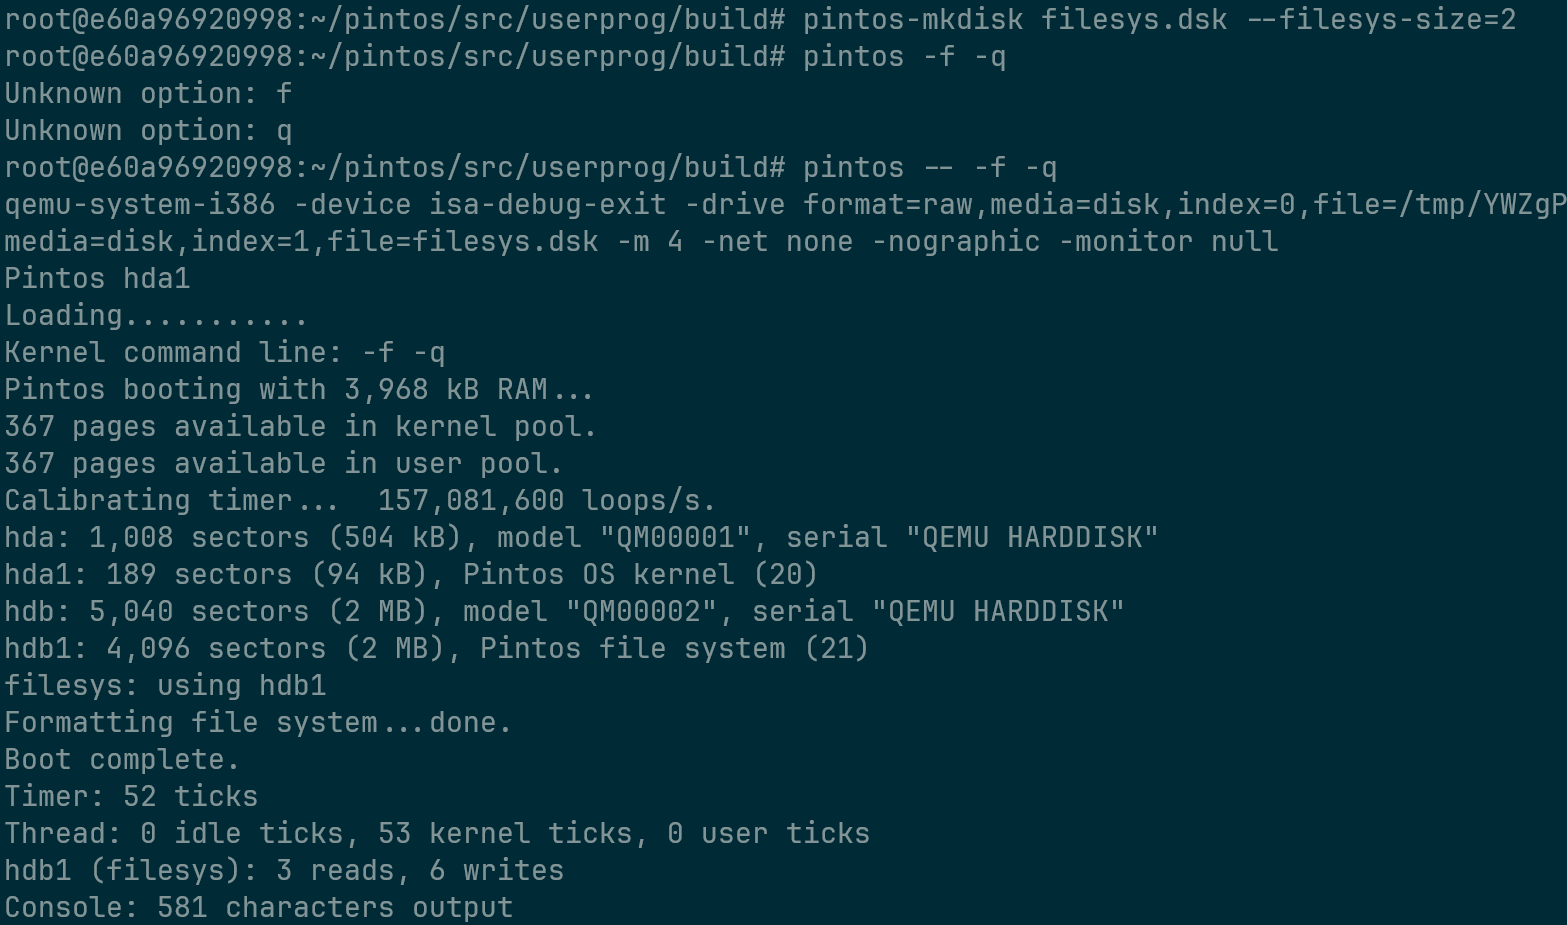
\includegraphics[width=0.7\textwidth]{img5/createfilesys.png}
    \caption{编译}
    \label{fig:make}
\end{figure}

注意到这里直接使用 \texttt{pintos -f -q} 会提示未知的参数,要修改为:\texttt{pintos -- -f -q},才能编译成功。

接下来,执行下一条命令,将 echo.c 复制到磁盘中,且命名为 echo。

\begin{figure}[H]
    \centering
    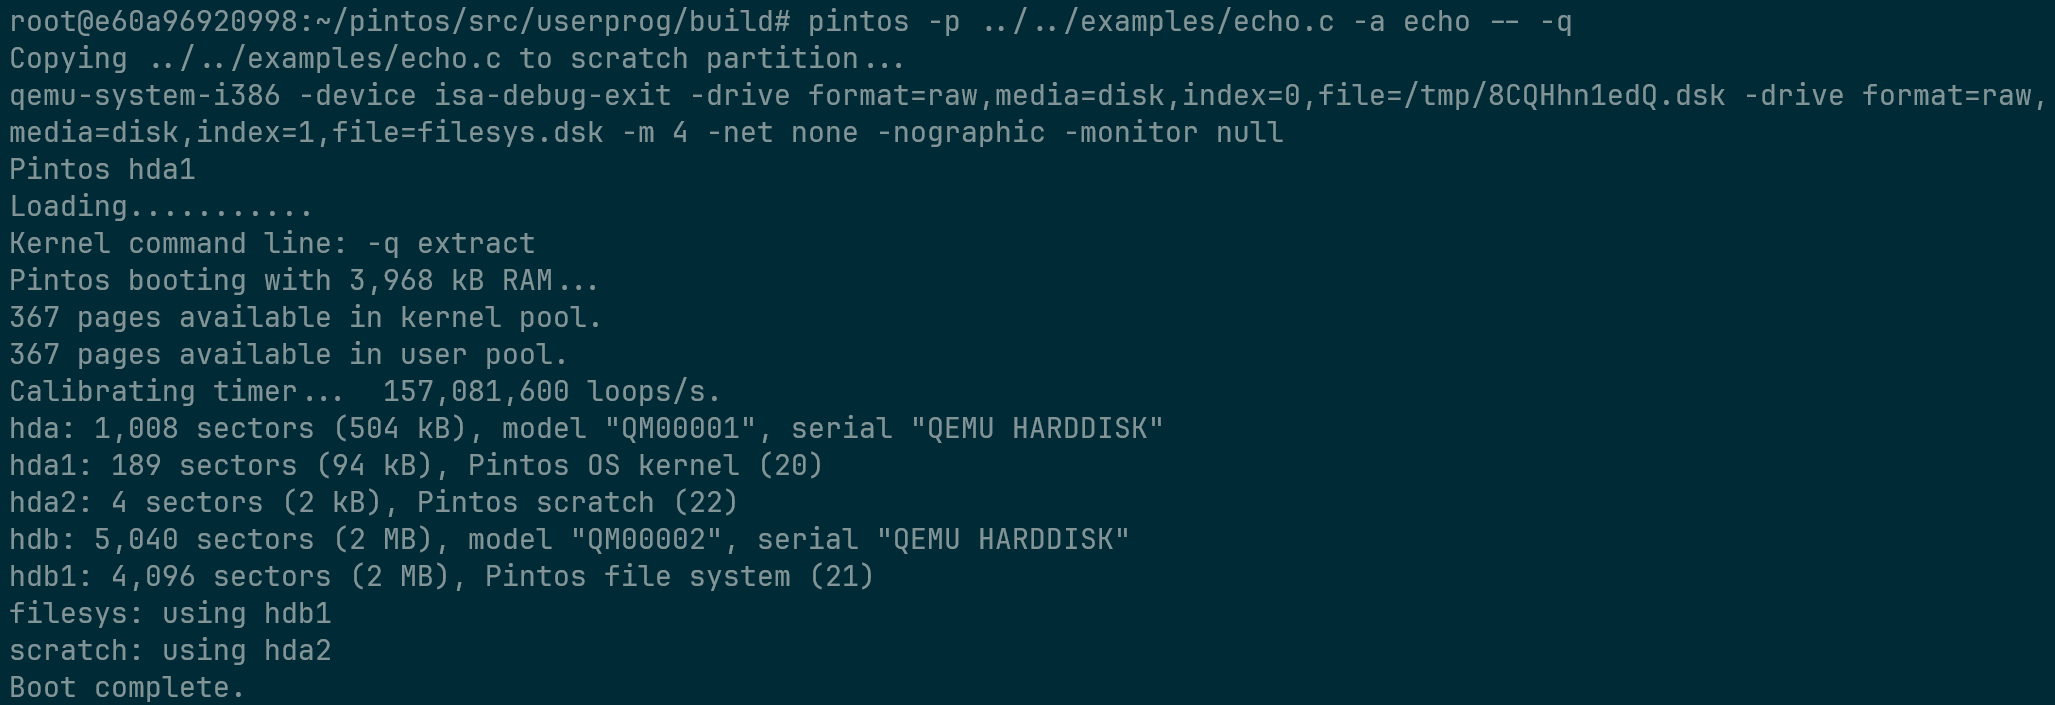
\includegraphics[width=0.8\textwidth]{img5/copy.png}
    \caption{复制文件}
    \label{fig:copyfile}
\end{figure}

在未实现参数传递时,我们直接执行 \texttt{pintos -- -q run 'echo x'} 这样的命令其实是很不合理的。
这个输入的含义是:执行echo文件,传递的参数是x。 实际上,echo x 被当成了一个整体来处理。

\begin{figure}[H]
    \centering
    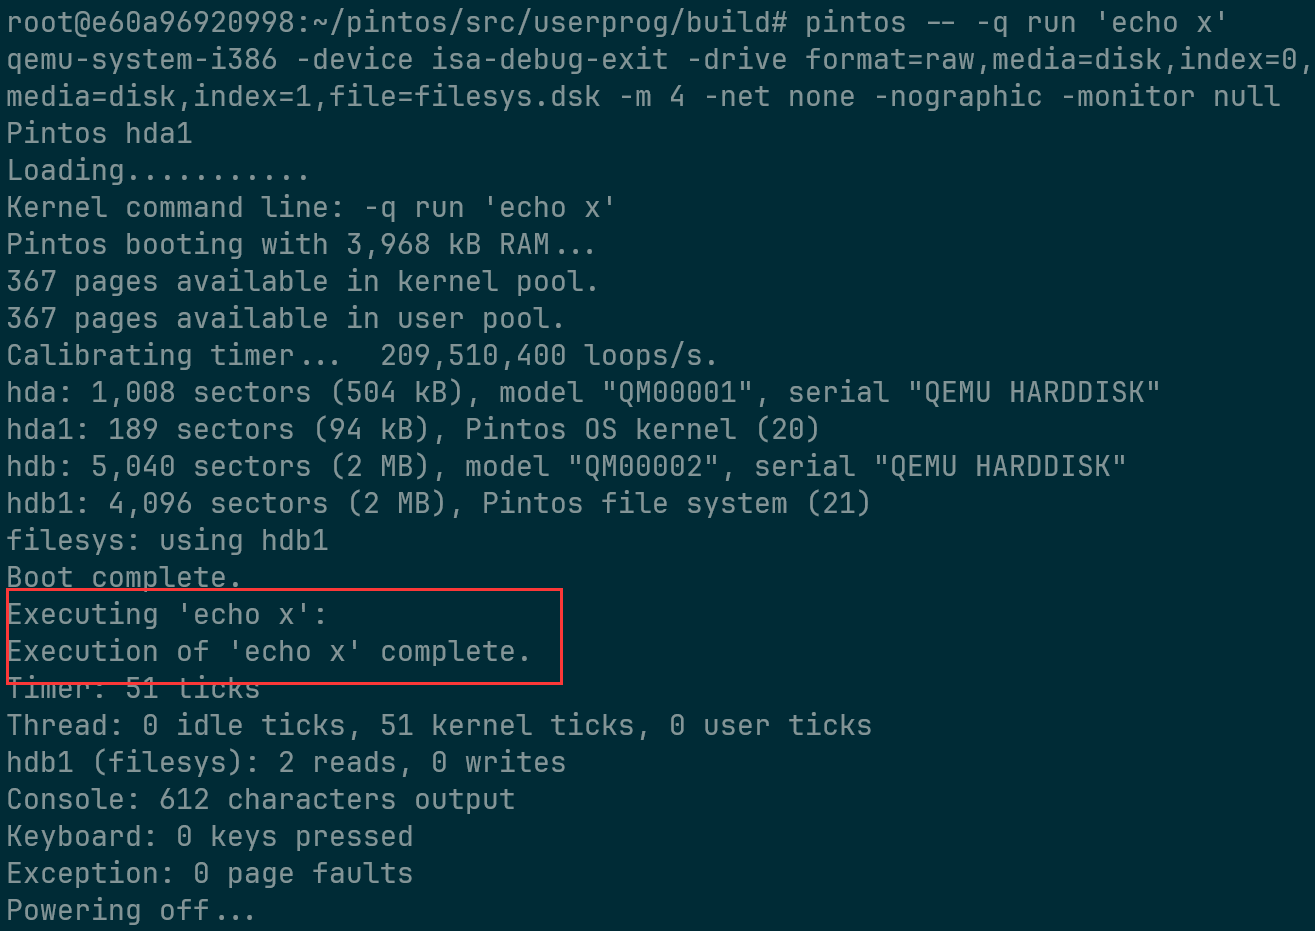
\includegraphics[width=0.65\textwidth]{img5/echo.png}
    \caption{Echo}
    \label{fig:echo}
\end{figure}

\subsection{开始分析代码}

先查看官方文档中对目前清空的介绍:

\begin{figure}[H]
    \centering
    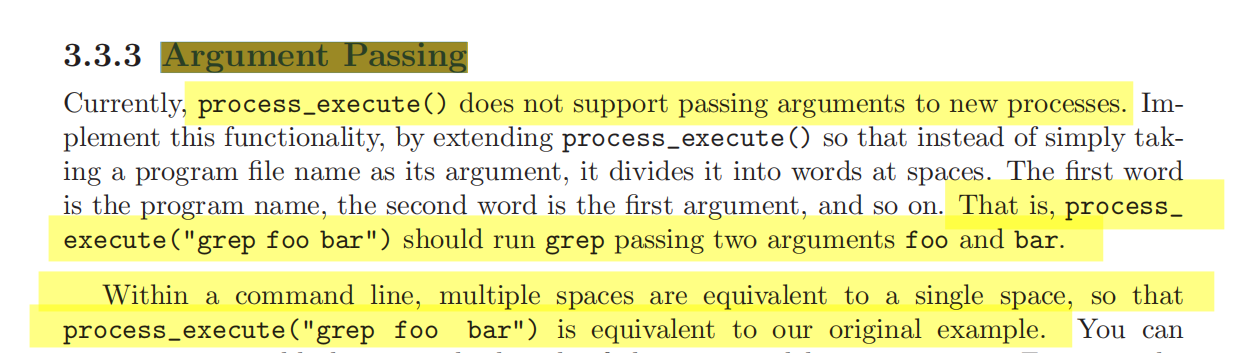
\includegraphics[width=0.8\textwidth]{img5/ref.png}
    \caption{Pintos References}
    \label{fig:ref}
\end{figure}

\begin{mdframed}
    翻译如下:
    
    目前,process\_execute()不支持向新进程传递参数。
通过扩展process\_execute()来实现此功能,而不是简单的task。
将程序filename作为其参数,它在空格处将其拆分为单词。第一个词
是程序名,第二个单词是第一个参数,以此类推。也就是.process
execute(“grep-foo-bar”)应该运行grep,传递两个参数foo和bar。
在命令行中多个空格相当于一个空格,以便进程执行(“grep-foo-bar”)与我们最初的示例等效。
\end{mdframed}

查看相关的代码处,我们可以看到以下内容:

\begin{lstlisting}[language=C,title=process]
    tid_t process_execute (const char *file_name) {
      char *fn_copy;
      tid_t tid;
    
      /* Make a copy of FILE_NAME.
         Otherwise there's a race between the caller and load(). */
      fn_copy = palloc_get_page (0);
      if (fn_copy == NULL)
        return TID_ERROR;
      strlcpy (fn_copy, file_name, PGSIZE);
    
      /* Create a new thread to execute FILE_NAME. */
      tid = thread_create (file_name, PRI_DEFAULT, start_process, fn_copy);
      if (tid == TID_ERROR)
        palloc_free_page (fn_copy); 
      return tid;
    }
\end{lstlisting}

\begin{ctt}
在传递参数时,传递 \texttt{process\_execute} 函数的参数 \texttt{file\_name} 既包括
可执行文件的名称,也包含了可执行文件的参数。
所以,要做的第一件事就是换把可执行文件名称和参数互相分开。
我们可以使用 \texttt{string.h} 中的 \texttt{strtok\_r()} 来分离参数。
\end{ctt}

\begin{lstlisting} [language=C,title=process]
    tid_t process_execute (const char *file_name) {
      char *fn_copy;
      char *thread_name;
      char *save_ptr; // 用来保存strtok_r的状态
    
      thread_name = malloc(strlen(file_name) + 1);
      strlcpy(thread_name, file_name, strlen(file_name) + 1);
      // 拷贝 file_name 到动态分配的 thread_name,以便后续通过 strtok_r 截取线程名称
      thread_name = strtok_r(thread_name, " ", &save_ptr); // 创建一个线程用来运行"文件名"
      tid_t tid;
    
      /* Make a copy of FILE_NAME.
         Otherwise there's a race between the caller and load(). */
      fn_copy = palloc_get_page (0);
      if (fn_copy == NULL)
        return TID_ERROR;
      strlcpy (fn_copy, file_name, PGSIZE);
    
      /* Create a new thread to execute FILE_NAME. */
      tid = thread_create (file_name, PRI_DEFAULT, start_process, fn_copy);
      free(thread_name); // 释放由 malloc 创建的线程名
      if (tid == TID_ERROR)
        palloc_free_page (fn_copy); 
      return tid;
    }
\end{lstlisting}

\begin{ctt}
这里我们首先在最开始添加两个 char *类型变量,\texttt{*save\_ptr} 指向
\texttt{file\_name} 的一个拷贝,是为了实现保存从命令语句中分离出来的真正的可执行文
件名,给 fn 分配与命令语句容量相等的内存空间。
\end{ctt}

\subsubsection{分析 start\_process()}

我们在函数中将 \texttt{file\_name} 通过 load 存储到栈中。

下面这个是 Pintos 中的原始代码。

\begin{lstlisting} [language=C,title=start\_process]
    static void
    start_process (void *file_name_)
    {
      char *file_name = file_name_;
      struct intr_frame if_;
      bool success;
    
      /* Initialize interrupt frame and load executable. */
      memset (&if_, 0, sizeof if_);
      if_.gs = if_.fs = if_.es = if_.ds = if_.ss = SEL_UDSEG;
      if_.cs = SEL_UCSEG;
      if_.eflags = FLAG_IF | FLAG_MBS;
      success = load (file_name, &if_.eip, &if_.esp);
    
      /* If load failed, quit. */
      palloc_free_page (file_name);
      if (!success) 
        thread_exit ();
    
      /* Start the user process by simulating a return from an
         interrupt, implemented by intr_exit (in
         threads/intr-stubs.S).  Because intr_exit takes all of its
         arguments on the stack in the form of a `struct intr_frame',
         we just point the stack pointer (%esp) to our stack frame
         and jump to it. */
      asm volatile ("movl %0, %%esp; jmp intr_exit" : : "g" (&if_) : "memory");
      NOT_REACHED ();
    }
\end{lstlisting}

修改后的代码如下所示:

\begin{lstlisting}[ language=C,title=process ]
    char *token, *save_ptr;
    file_name = strtok_r(file_name, " ", &save_ptr); // 获取文件名
    success = load (file_name, &if_.eip, &if_.esp);
\end{lstlisting}

\subsubsection{分析 load() 函数}

主要是将从FILE\_NAME获取的可执行的程序放入到当前线程中。

针对传参,我们需要第二次参数分离:传递过来的是\texttt{file\_name="args-single onearg"}。

\begin{lstlisting}[language=C, title= load]
    /* Separate file name and arguments. */
    char *exec_name;
    char *save_ptr;
  
    /* Make a modifiable copy of file_name. */
    char modifiable_file_name[PGSIZE];
    strlcpy(modifiable_file_name, file_name, PGSIZE);
  
    /* Extract the executable name (first token). */
    exec_name = strtok_r(modifiable_file_name, " ", &save_ptr);
  
    /* Open the executable file. */
    file = filesys_open(exec_name);
    if (file == NULL) 
    {
      printf ("load: %s: open failed\n", exec_name);
      goto done; 
    }
\end{lstlisting}

另外,在 load() 函数中,注释中写明了 \texttt{setup\_stack()} 函数的作用是设置参数堆栈。

\begin{figure}[H]
    \centering
    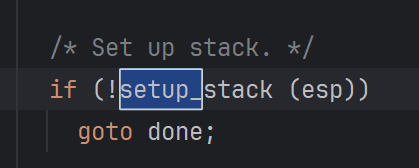
\includegraphics[width=0.3\textwidth]{img5/setup.png}
    \caption{load()}
    \label{fig:load}
\end{figure}

而在 \texttt{setup\_stack()} 函数中,它仅仅实现了页的初始化,并没有参数传递实现的代码。

因此我们需要将用strok分离出的filename以及argv传递进去。

一个实现思路是,在 \texttt{setup\_stack()} 函数中添加参数 \texttt{file\_name} 和 \texttt{save\_ptr}

\begin{figure}[H]
    \centering
    \begin{subfigure}[b]{0.45\textwidth}
        \centering
        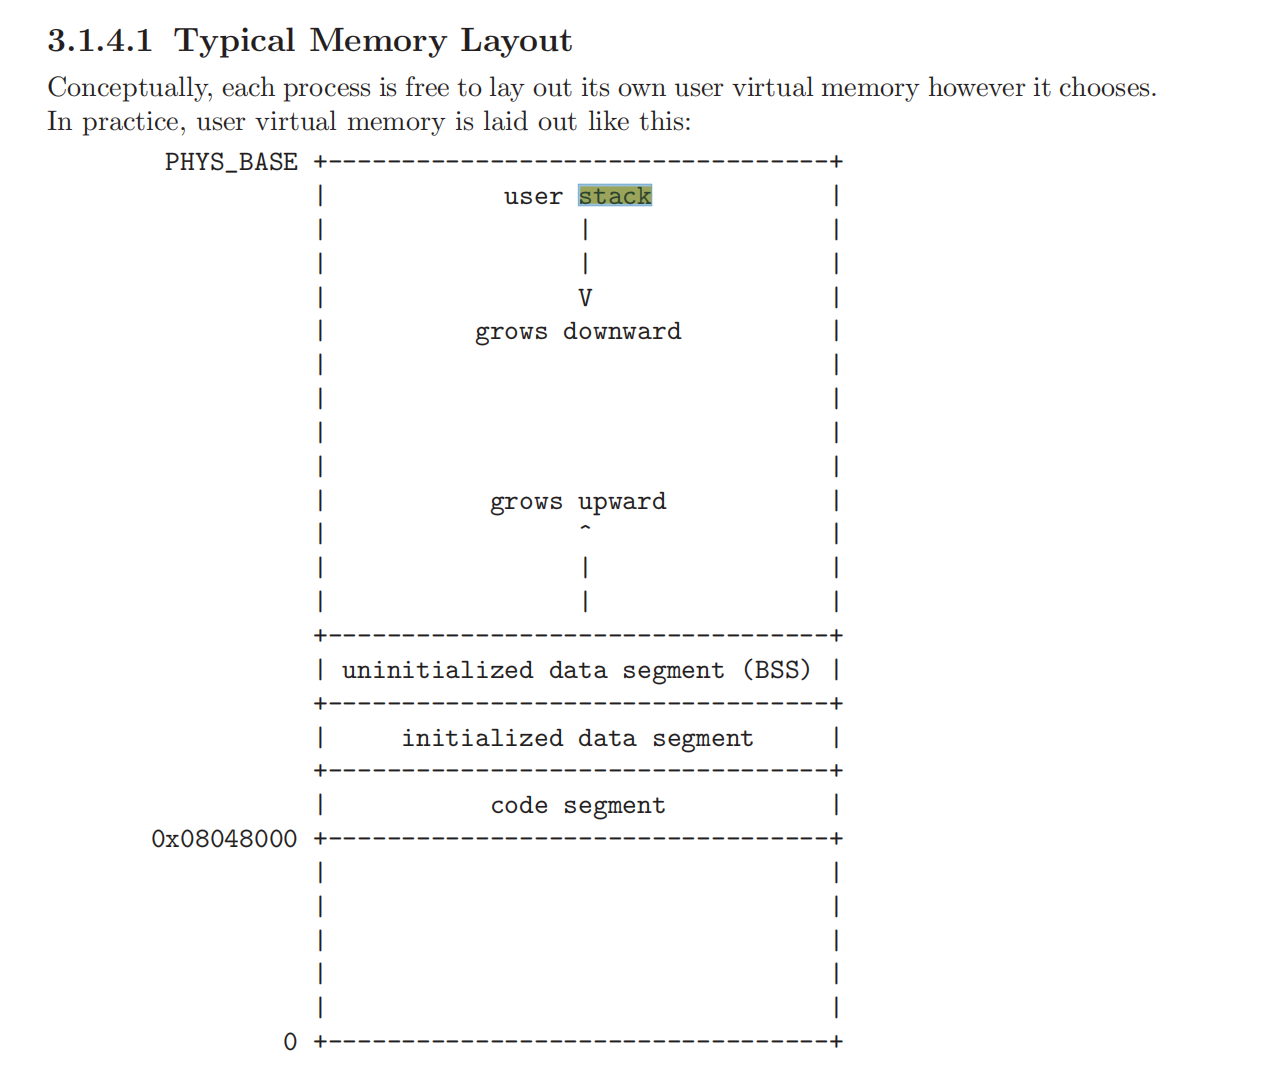
\includegraphics[width=\textwidth]{img5/stack.png}
        \label{fig:left_stack}
    \end{subfigure}
    \hfill
    \begin{subfigure}[b]{0.42\textwidth}
        \centering
        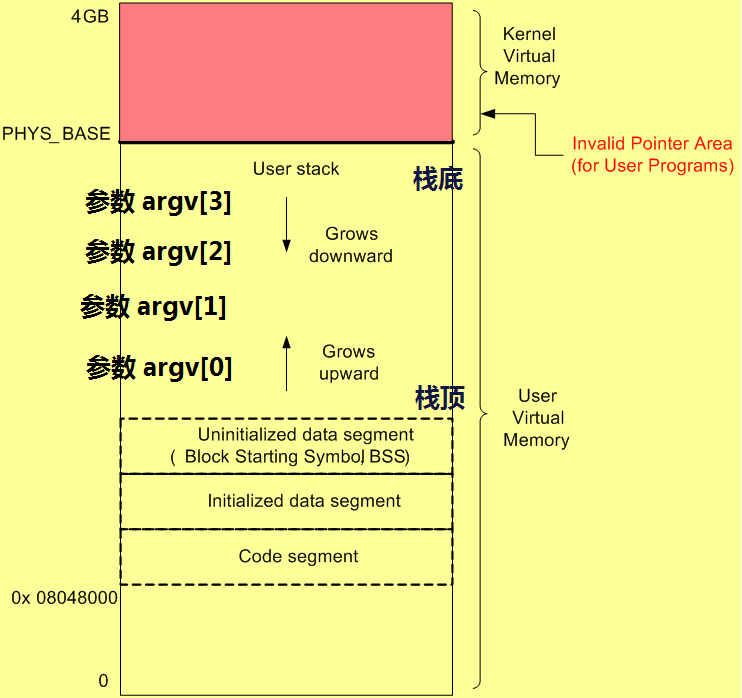
\includegraphics[width=\textwidth]{img5/stackover.png}
        \label{fig:right_stack}
    \end{subfigure}
    \label{fig:stack_subfigures}
\end{figure}

\begin{ctt}
\textbf{if\_.esp} 原来指向esp的内核和用户区边界为避免内存访问越界(访问到内核区)

所以需将\texttt{setup\_stack()}函数中的\texttt{esp = PHYS\_BASE}
修改成 \texttt{*esp = PHYS\_BASE - 12;}

后来,文档中还附加了一条对于 \textbf{bin/ls -l foo bar} 命令执行时栈的增长情况:
\end{ctt}

\begin{figure}[H]
    \centering
    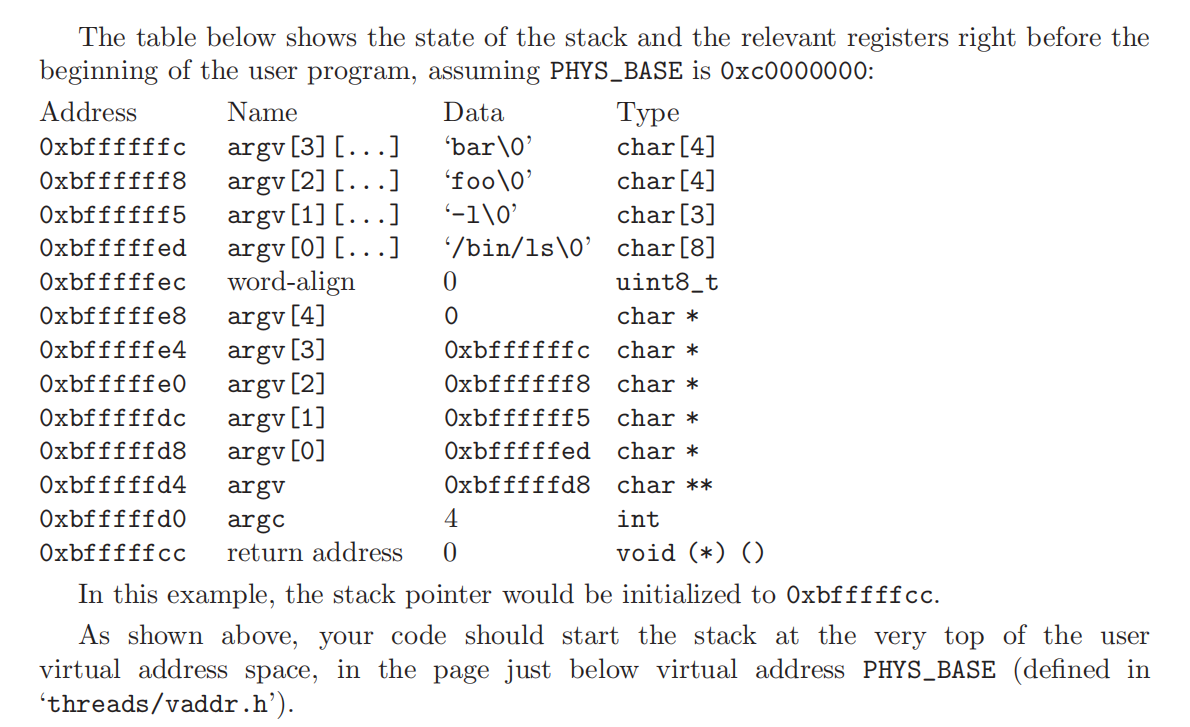
\includegraphics[width=0.55\textwidth]{img5/example.png}
    \caption{示例栈增长}
    \label{fig:ls}
\end{figure}

根据 PPT 上的提示,我们编写以下代码来实现初始化栈:

另外,官方文档中还提到了我们可以使用 \textbf{hex\_dump()} 函数来打印此时栈的信息,不妨添加进去。

\begin{figure}[H]
    \centering
    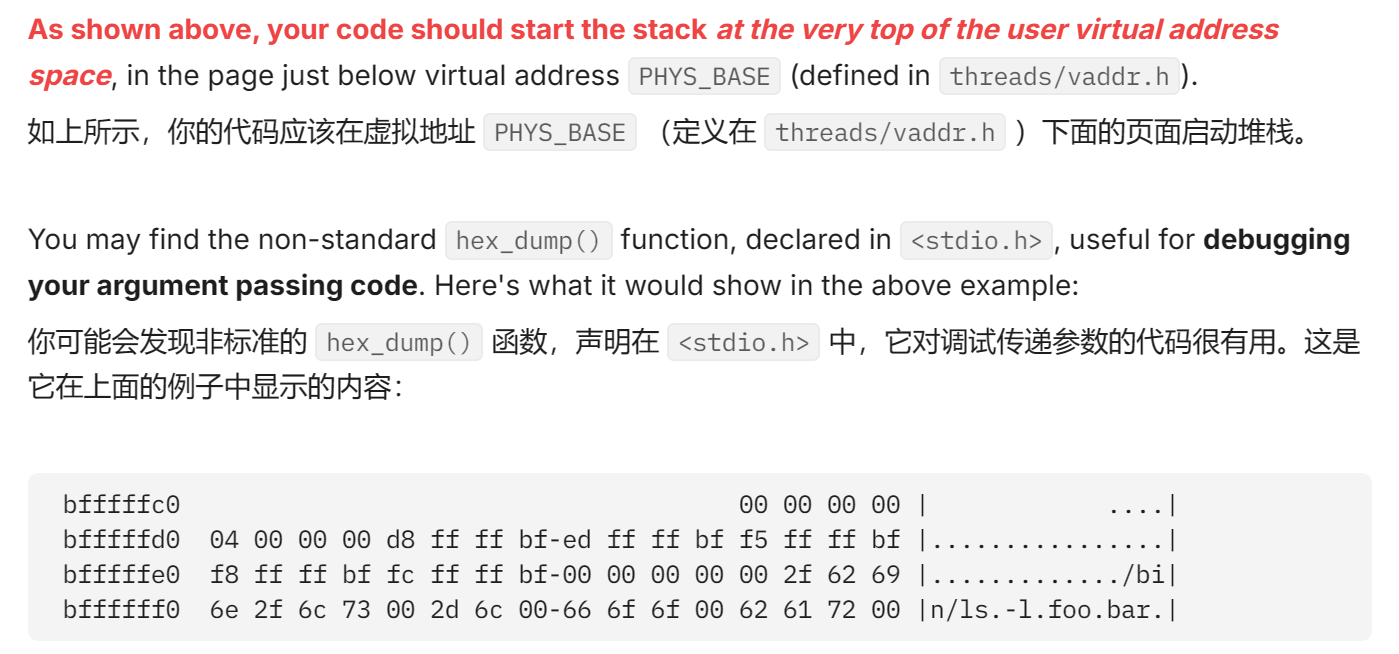
\includegraphics[width=0.5\textwidth]{img5/tips.png}
    \caption{hex\_dump()}
    \label{fig:hex}
\end{figure}

在函数中,写好了为什么要用这样的方式实现的具体注释:

\begin{lstlisting}[language=C, title= setup\_stack]
    static bool
    setup_stack (void **esp, char* file_name)
    {
      uint8_t *kpage;
      bool success = false;
    
      // 分配一页用户内存并将其安装到用户栈的顶部
      kpage = palloc_get_page (PAL_USER | PAL_ZERO);
      if (kpage != NULL) 
        {
          success = install_page (((uint8_t *) PHYS_BASE) - PGSIZE, kpage, true);
          if (success)
            *esp = PHYS_BASE - 12;  // 初始化栈指针到栈顶
          else
            palloc_free_page (kpage);
        }
    
      // 创建一个临时拷贝的文件名字符串
      char *token, *temp_ptr;
      char *filename_cp = malloc(strlen(file_name) + 1);
      strlcpy (filename_cp, file_name, strlen(file_name) + 1);
    
      // 计算参数数量 (argc)
      enum intr_level old_level = intr_disable();
      int argc = 1; // 初始值为 1,因为至少有一个参数
      bool is_lastone_space = false; // 记录最后一个字符是否为空格
      for (int j = 0; j != strlen(file_name); j++) {
        if (file_name[j] == ' ') {
          if (!is_lastone_space)
            argc++; // 如果遇到新的空格且不是连续空格,参数计数加一
          is_lastone_space = true;
        } else {
          is_lastone_space = false;
        }
      }
      intr_set_level (old_level);
    
      // 为参数指针 (argv) 分配内存
      int *argv = calloc(argc, sizeof(int));
    
      // 将文件名分割为各个参数,并依次压入栈中
      int i;
      token = strtok_r (file_name, " ", &temp_ptr);
      for (i = 0; ; i++) {
        if (token) {
          *esp -= strlen(token) + 1; // 为参数字符串分配空间
          memcpy(*esp, token, strlen(token) + 1); // 将参数字符串复制到栈
          argv[i] = *esp; // 保存参数地址
          token = strtok_r (NULL, " ", &temp_ptr); // 获取下一个参数
        } else {
          break; // 没有更多参数时退出循环
        }
      }
    
      // 对齐到 4 字节边界 (Word Align)
      *esp -= ((unsigned)*esp % 4);
    
      // 空指针标志 (null pointer sentinel),表示 argv[argc] 为空
      *esp -= sizeof(int);
    
      // 将参数地址依次压入栈中
      for (i = argc - 1; i >= 0; i--)
      {
        *esp -= sizeof(int);
        memcpy(*esp, &argv[i], sizeof(int));
      }
    
      // 压入 argv 的地址
      int tmp = *esp;
      *esp -= sizeof(int);
      memcpy(*esp, &tmp, sizeof(int));
    
      // 压入 argc (参数数量)
      *esp -= sizeof(int);
      memcpy(*esp, &argc, sizeof(int));
    
      // 压入返回地址 (return address)
      *esp -= sizeof(int);
      memcpy(*esp, &argv[argc], sizeof(int));
    
      // 打印栈的状态,便于调试
      printf("STACK SET. ESP: %p\n", esp);
      hex_dump((uintptr_t)esp, esp, 100, true); // 打印栈中前 100 字节的数据,便于调试
    
      // 释放临时分配的内存
      free(filename_cp);
      free(argv);
    
      return success;
    }
    
\end{lstlisting}

\begin{ctt}
    在官方文档中提到,栈的增长是反方向的:栈地址是向下增长的,而字符串的地址是向上增长的,所以在放
    置参数的时候需要把参数倒序放置。
\end{ctt}

直到这里,即使我们使用 \textbf{make check} 命令,仍然无法看到输出,只会出现:

\begin{mdframed}
    Run didn’t produce any output”。
\end{mdframed}

因为用户程序的打印(输出到 stdout)也是通过写的系统调用实现的。

\begin{figure}[H]
    \centering
    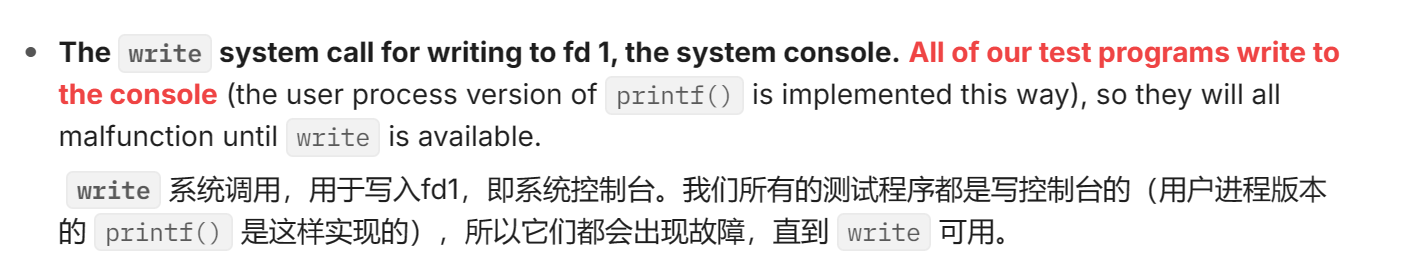
\includegraphics[width=0.5\textwidth]{img5/write.png}
    \caption{write()}
    \label{fig:fail}
\end{figure}

\subsection{实现系统调用}

除了我们要实现的 \texttt{userprog/syscall.c},在 \texttt{lib/user} 文件夹下,还有一对 \texttt{syscall.h} 和 \texttt{syscall.c} 文件

\begin{ctt}
这组文件,是 提供给用户的系统调用接口,其通过 int \$0x30 
中断指令以唤起一个系统调用,
最终会落入 userprog/syscall.c 的 syscall\_handler() 函数中。
\end{ctt}

其 enum 中定义了不同的系统调用的序号:

\begin{lstlisting}[language=C, title= syscall.h]
    enum {
        /* Projects 2 and later. */
        SYS_HALT,                   /**< Halt the operating system. */
        SYS_EXIT,                   /**< Terminate this process. */
        SYS_EXEC,                   /**< Start another process. */
        SYS_WAIT,                   /**< Wait for a child process to die. */
        SYS_CREATE,                 /**< Create a file. */
        SYS_REMOVE,                 /**< Delete a file. */
        SYS_OPEN,                   /**< Open a file. */
        SYS_FILESIZE,               /**< Obtain a file's size. */
        SYS_READ,                   /**< Read from a file. */
        SYS_WRITE,                  /**< Write to a file. */
        SYS_SEEK,                   /**< Change position in a file. */
        SYS_TELL,                   /**< Report current position in a file. */
        SYS_CLOSE,                  /**< Close a file. */
    
        /* Project 3 and optionally project 4. */
        SYS_MMAP,                   /**< Map a file into memory. */
        SYS_MUNMAP,                 /**< Remove a memory mapping. */
    
        /* Project 4 only. */
        SYS_CHDIR,                  /**< Change the current directory. */
        SYS_MKDIR,                  /**< Create a directory. */
        SYS_READDIR,                /**< Reads a directory entry. */
        SYS_ISDIR,                  /**< Tests if a fd represents a directory. */
        SYS_INUMBER                 /**< Returns the inode number for a fd. */
      };
\end{lstlisting}

故我们需要在 \textbf{syscall\_handler()} 中实现分发:
根据类型分发给各个具体处理函数,逐个实现。
返回值要放在 EAX 中传回调用者。

\begin{ctt}
    在 Pintos 中,struct intr\_frame 是用来保存中断处理器状态的结构体。在系统调用返回时,通常会将结果值存储到 f->eax 中,因为这是 x86 架构的约定——返回值通过 eax 寄存器传递。
    
    \vspace{0.5cm}

    对于系统调用 SYS\_EXIT,需要返回一个退出码到用户进程,返回值就需要存放到 f->eax 中。
    类似地,SYS\_WRITE 也会将写入的字节数返回到 f->eax。
\end{ctt}

\begin{lstlisting}[language=C, title= syscall.c]
    static void syscall_handler (struct intr_frame *f UNUSED) {
        int *p = f->esp;
        is_valid_addr(p);
    
        int system_call = *p;
        switch (system_call) {
            case SYS_HALT: syscall_halt(); break;
            case SYS_EXIT: syscall_exit(f); break; // 直接关机,不需要返回值,故是 void function
            case SYS_EXEC: f->eax = syscall_exec(f); break;
            case SYS_WAIT: f->eax = syscall_wait(f); break;
            case SYS_CREATE: f->eax = syscall_creat(f); break;
            case SYS_REMOVE: f->eax = syscall_remove(f); break;
            case SYS_OPEN: f->eax = syscall_open(f); break;
            case SYS_FILESIZE: f->eax = syscall_filesize(f); break;
            case SYS_READ: f->eax = syscall_read(f); break;
            case SYS_WRITE: f->eax = syscall_write(f); break;
            case SYS_SEEK: syscall_seek(f); break; // 调整文件指针的位置,也不需要返回值
            case SYS_TELL: f->eax = syscall_tell(f); break;
            case SYS_CLOSE: syscall_close(f); break;
    
            default:
            printf("Default %d\n",*p);
        }
    }
\end{lstlisting}

在上方的函数中,有一些函数是不需要返回值的,这些 \texttt{void function} 在定义的时候要注意一下。

其次,Pintos 中已经使用了 \texttt{syscall\_init} 将中断处理函数注册到寄存器:

\begin{lstlisting}[language=C, title= init.c]
    void syscall_init (void) {
        intr_register_int (0x30, 3, INTR_ON, syscall_handler, "syscall");
    }
\end{lstlisting}

另外要注意的是,Pintos 中不允许在系统调用中使用 malloc() 函数:

\begin{figure}[H]
    \centering
    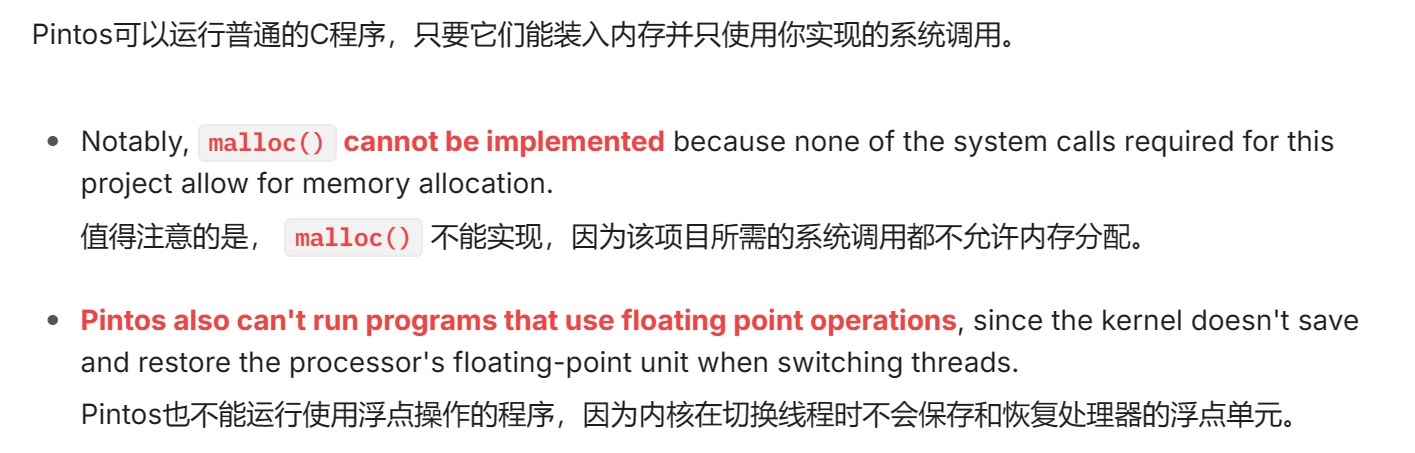
\includegraphics[width=0.5\textwidth]{img5/warning.png}
    \caption{malloc()}
    \label{fig:malloc}
    \end{figure}
\subsection{处理内存非法访问}

PPT 中的提示了使用 \textbf{syscall\_create} 来实现:

\begin{figure}[H]
    \centering
    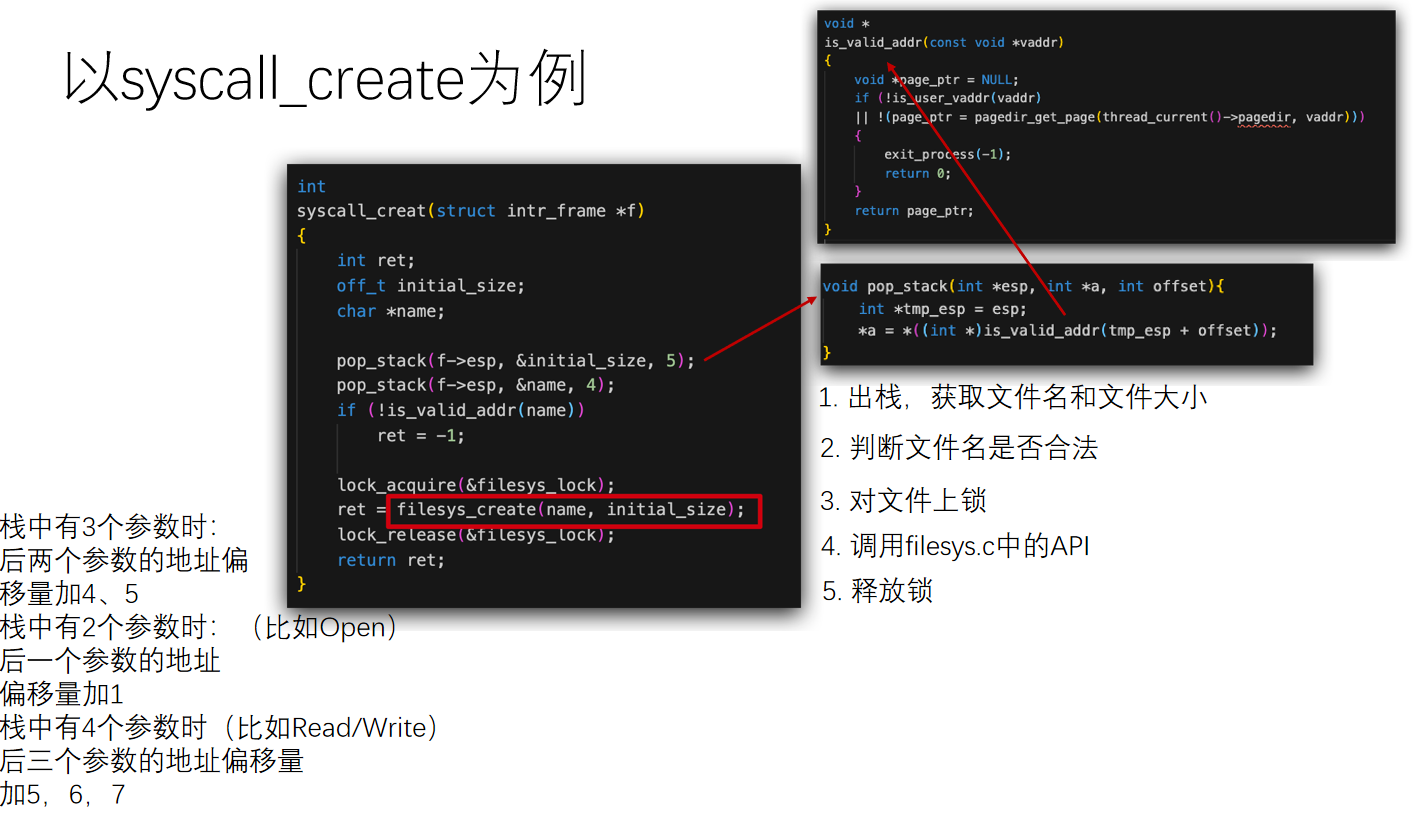
\includegraphics[width=0.8\textwidth]{img5/ppt.png}
    \caption{PPT}
    \label{fig:check}
\end{figure}

为了保证内核不受到破坏,需要立即终止发出非法指针请求的进程。查
看 \texttt{userprog/pagedir.c} 和 \texttt{threads/vaddr.h},可以发现已经为我们定义了以下两个函数:

\begin{lstlisting}[language=C,title= pagedir\_get\_page()]
    /* Looks up the physical address that corresponds to user virtual address UADDR in PD.
    Returns the kernel virtual address
    corresponding to that physical address, or a null pointer if UADDR is unmapped. */
    void *pagedir_get_page (uint32_t *pd, const void *uaddr) {
    uint32_t *pte;
    ASSERT (is_user_vaddr (uaddr));
    pte = lookup_page (pd, uaddr, false);
    if (pte != NULL && (*pte & PTE_P) != 0)
        return pte_get_page (*pte) + pg_ofs (uaddr);
    else
        return NULL;
   }
\end{lstlisting}

\begin{lstlisting}[language=C,title= is\_user\_vaddr()]
    /* Returns true if VADDR is a user virtual address. */
    static inline bool is_user_vaddr (const void *vaddr) {
        return vaddr < PHYS_BASE;
    }
\end{lstlisting}

除了空指针以外,这就是最常见的两个异常情况。当出现异常的时候都会返回异常信息。
可以借助这两个函数来实现内存访问的安全控制。

我们可以跟着这个思路来编写代码:

\begin{lstlisting}[language=C, title= syscall\_create()]
    // 检查传入的虚拟地址是否是用户空间的有效地址:
    // 使用 is_user_vaddr 判断地址是否在用户地址范围内。如果是有效的用户地址,则使用 pagedir_get_page 从当前线程的页目录中获取该虚拟地址对应的物理页指针。
    // 如果地址无效或无法找到对应的物理页,则调用 exit_process(-1) 退出当前进程。

    void *is_valid_addr(const void *vaddr) {
        void *page_ptr = NULL;
        if (!is_user_vaddr(vaddr) || !(page_ptr = pagedir_get_page(thread_current()->pagedir, vaddr))) {
            // 地址无效,退出进程
            exit_process(-1);
            return 0;
        }
    // 地址有效,返回物理页指针
    return page_ptr;
    }
\end{lstlisting}

如果地址无效则以异常状态中止进程,有效则返回物理地址。

再编写 pop\_stack() 函数,用于从栈中取得元素,方便取得参数:

\begin{lstlisting}[language=C, title= pop\_stack()]
    void pop_stack(int *esp, int *a, int offset){
        int *tmp_esp = esp;
        *a = *((int *)is_valid_addr(tmp_esp + offset));
    }
\end{lstlisting}

这里是因为 Pintos 使用的是 4 字节对齐,所以 offset 参数可以方便地使用整数来取得参数。

\begin{figure}[H]
    \centering
    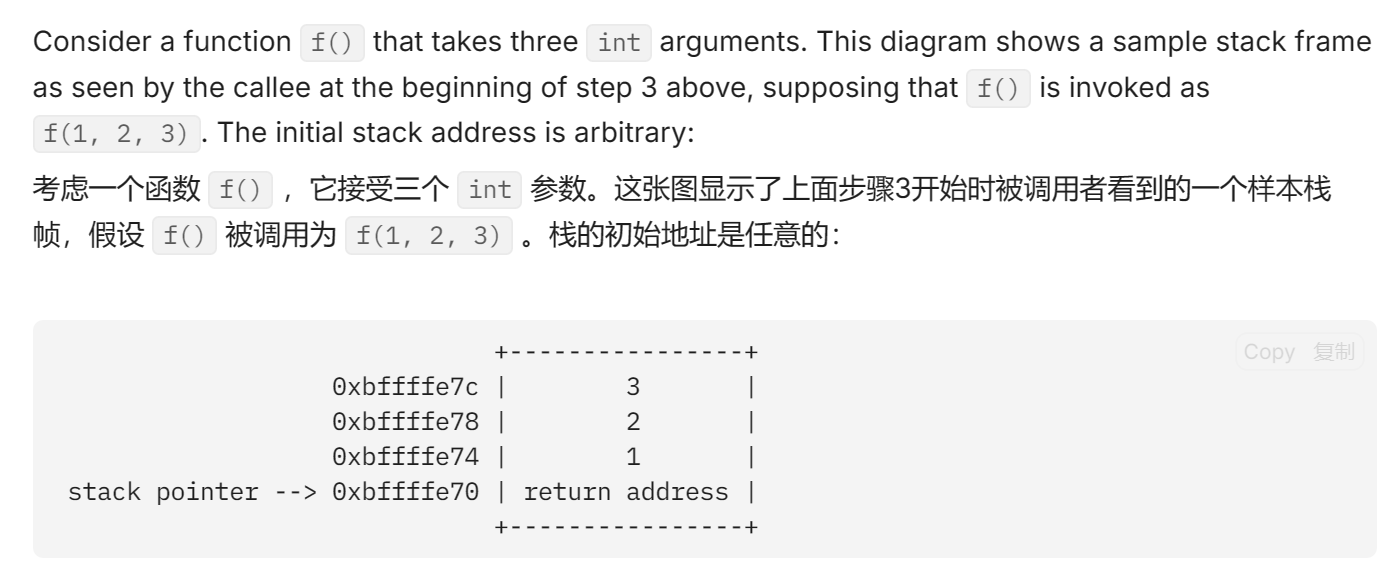
\includegraphics[width=0.5\textwidth]{img5/stackpointer.png}
    \caption{栈指针}
    \label{fig:stack}
\end{figure}

\subsection{完善系统调用}

按照 PPT 要求,在 \texttt{thread.h} 中新增结构体变量:

\begin{figure}[H]
    \centering
    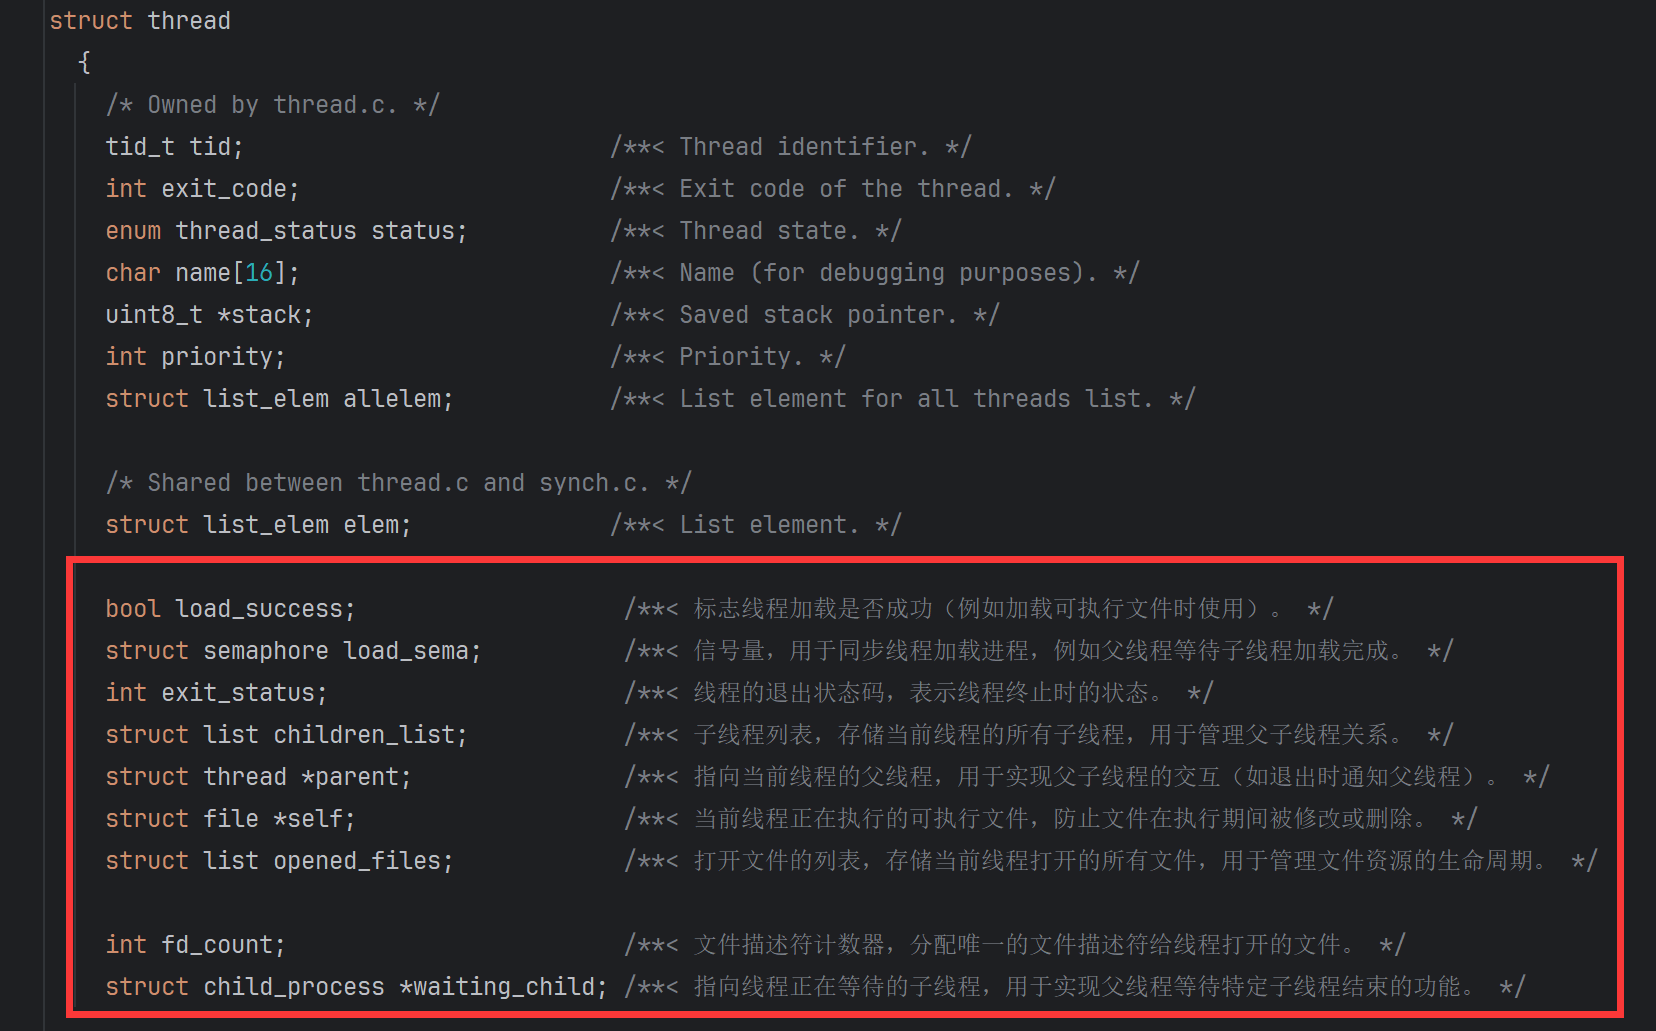
\includegraphics[width=0.8\textwidth]{img5/new.png}
    \caption{thread.h}
    \label{fig:thread}
\end{figure}

同时定义全局锁:\textbf{struct lock filesys\_lock},用于文件系统操作的同步。该结构体 \texttt{lock} 位于 \textbf{synch.h} 中。

当然,不能忘记了子进程的结构体定义:

\begin{lstlisting}[language=C,title= child\_process]
struct child_process {
    int tid;                     /**< 子进程的线程 ID。 */
    bool if_waited;              /**< 子进程是否已被父进程等待。 */
    int exit_status;             /**< 子进程的退出状态。 */
    struct list_elem child_elem; /**< 子进程的元素。 */
    struct semaphore wait_sema;  /**< 等待子进程退出的信号量。 */
};
\end{lstlisting}

\subsubsection{halt}

这里只需要简单地调用 \textbf{devices/shutdown.c} 下的函数接口即可:

\begin{lstlisting}[language=C]
    void syscall_halt(void){
        shutdown_power_off();
    }
\end{lstlisting}

\subsection{syscall\_exit}

\begin{lstlisting} [language=C]
static void syscall_exit(struct intr_frame *f) {
    // exit_code在系统调用之后被解析为参数
    int exit_code = *(int *)check_read_user_ptr(f->esp + ptr_size, sizeof(int));
    thread_current()->exit_status = exit_code;
    thread_exit();
}
\end{lstlisting}

\vspace{0.8cm}

\begin{ctt}
\texttt{syscall\_exit} 函数实现了系统调用,用于终止当前进程。
通过遍历查找对应的子进程描述结构(\texttt{child\_process}),
更新其退出状态码(\texttt{exit\_status})以及是否已被父线程等待的标志(\texttt{if\_waited})。
同时,将当前线程的退出状态存储在其自身的 \texttt{exit\_status} 字段中。
为了避免多线程环境下的竞争问题,函数通过禁用中断(\texttt{intr\_disable})确保状态更新的原子性。

\vspace{0.5cm}

最后调用 \texttt{thread\_exit} 终止当前线程,之所以选择 \texttt{thread\_exit} 而非直接调用 \texttt{process\_exit},
是因为前者还包含了对信号量的同步操作,并且可以用于终止用户进程和系统线程。
\end{ctt}

\vspace{0.8cm}

其中,子函数 \texttt{exit\_process} 的实现如下:

\begin{lstlisting}[language=C]
    void exit_process(int status) {
        struct child_process *cp;
        struct thread *cur_thread = thread_current();
        enum intr_level old_level = intr_disable(); // 禁用中断以保证线程状态更新的安全性。
    
        // 遍历当前线程的父线程的子线程列表,更新当前线程在父线程记录中的状态。
        for (struct list_elem *e = list_begin(&cur_thread->parent->children_list);
             e != list_end(&cur_thread->parent->children_list);
             e = list_next(e)) {
            cp = list_entry(e, struct child_process, child_elem);
            if (cp->tid == cur_thread->tid) {
                cp->if_waited = true;       // 标记当前线程已被父线程等待过。
                cp->exit_status = status;  // 更新退出状态。
            }
        }
        cur_thread->exit_status = status;  // 设置当前线程的退出状态。
        intr_set_level(old_level); // 恢复中断状态
        thread_exit(); // 退出当前线程
    }
\end{lstlisting}

\subsection{syscall\_exec}

\begin{lstlisting}[language=C]
    // 运行其名称在 cmd_line 中给出的可执行文件,并传递任何给定的参数,返回新进程的进程ID(pid)
    static void syscall_exec(struct intr_frame *f) {
        char *cmd_line = *(char **)check_read_user_ptr(f->esp + ptr_size, ptr_size);
        check_read_user_str(cmd_line);
        f->eax = process_execute(cmd_line);
    }
\end{lstlisting}

\vspace{0.7cm}

\begin{ctt}
    \texttt{syscall\_exec} 函数实现了 exec 系统调用,
    用于运行用户程序指定的可执行文件并传递命令行参数。
    函数首先从用户栈中读取命令行字符串(\texttt{cmd\_line}),这是用户程序传递的参数。

    \vspace{0.4cm}

    随后,通过 \texttt{check\_read\_user\_ptr}验证命令行指针是否合法,
    确保指针指向的地址位于用户空间内,
    并进一步使用 \texttt{check\_read\_user\_str} 验证字符串的内容是否安全可读,防止非法内存访问。
    验证通过后,函数调用 \texttt{process\_execute}(\texttt{cmd\_line}),
    用于创建新进程并执行命令行中指定的程序。\texttt{process\_execute} 返回新进程的进程 ID(pid),
    代表子进程的唯一标识符,函数将其存储在中断帧的 eax 寄存器中,供用户程序访问。
\end{ctt}

\subsection{syscall\_wait}

\begin{lstlisting}[language=C, title= syscall\_wait()]
    int syscall_wait(struct intr_frame *f) {
        tid_t child_tid;
        pop_stack(f->esp, &child_tid, 1);  // Extract the child process ID from the user stack.
        return process_wait(child_tid);   // Wait for the child process and return its exit status.
    }
\end{lstlisting}

\begin{ctt}
    \texttt{syscall\_wait} 实现了 WAIT 系统调用,用于当前进程等待一个指定的子进程完成执行。它通过中断帧的栈指针(f->esp)从用户栈中获取传递的子进程线程 ID(tid)。
\end{ctt}



在未实现 \texttt{syscall\_write} 之前,会出现这样的情况:

\begin{figure}[H]
    \centering
    \begin{subfigure}[b]{0.45\textwidth}
        \centering
        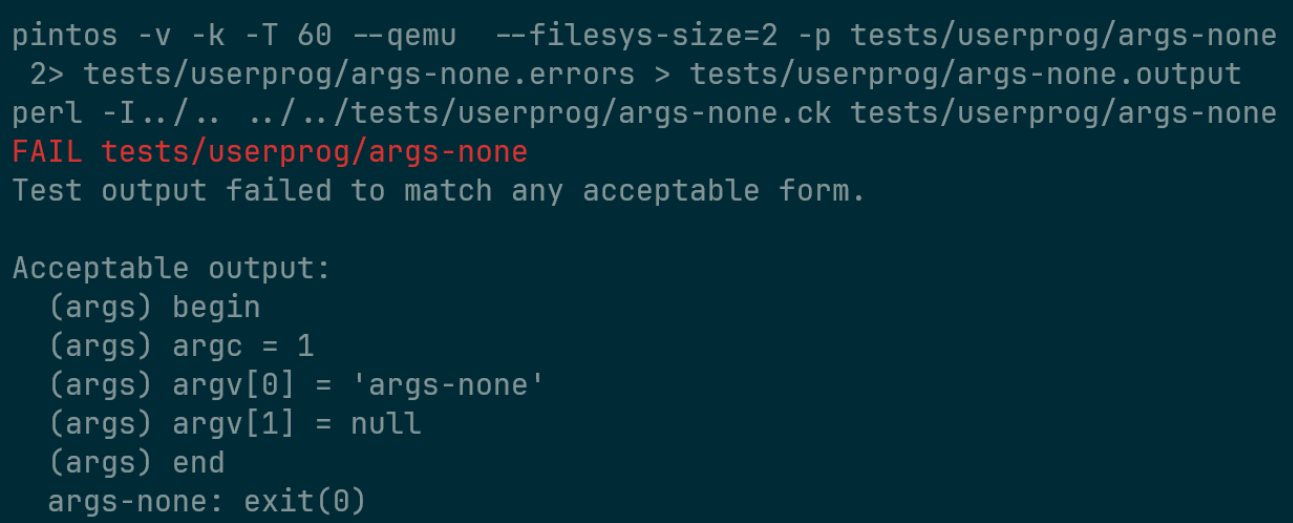
\includegraphics[width=\textwidth]{img5/failed1.png}
        \label{fig:failed1}
    \end{subfigure}
    \hfill
    \begin{subfigure}[b]{0.45\textwidth}
        \centering
        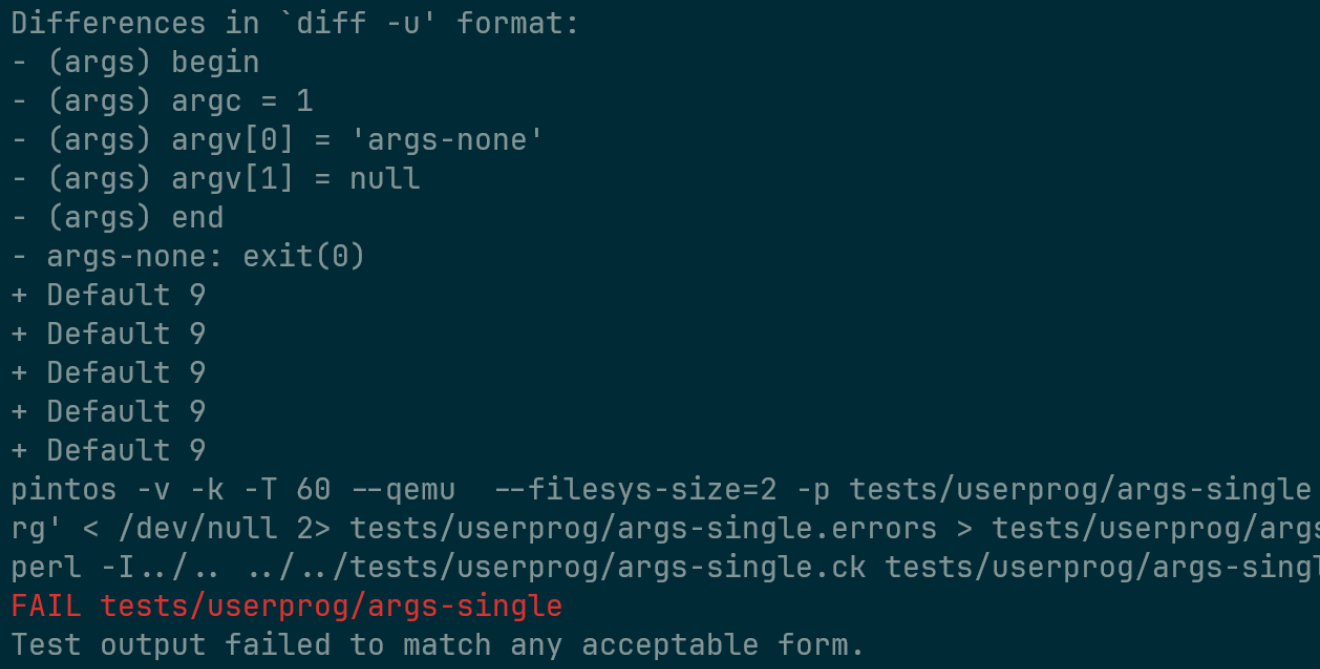
\includegraphics[width=\textwidth]{img5/failed2.png}
        \label{fig:failed2}
    \end{subfigure}
    \caption{Combination of Failed Results}
    \label{fig:failed_results}
\end{figure}


输出的结果显示为:\textbf{Default 9} 这在 \texttt{user/syscall.c} 中是 9 号, \texttt{SYS\_WRITE},用户程序的打印(输出到 stdout)也是通过写的系统调用实现的。

\subsubsection{syscall\_write}

\begin{lstlisting}[language=C, title= syscall\_write()]
    int syscall_write(struct intr_frame *f) {
        int ret;                  /**< 写入操作的返回值。 */
        int size;                 /**< 要写入的数据大小(字节)。 */
        void *buffer;             /**< 数据缓冲区的起始地址。 */
        int fd;                   /**< 文件描述符。 */
    
        // 从用户栈中读取系统调用参数,分别是 size、buffer 和 fd
        pop_stack(f->esp, &size, 7);
        pop_stack(f->esp, &buffer, 6);
        pop_stack(f->esp, &fd, 5);
    
        // 检查 buffer 是否为有效的用户地址
        if (!is_valid_addr(buffer))
            ret = -1;

        // 如果文件描述符是标准输出(fd == 1),直接将数据输出到控制台
        if (fd == 1) {
            putbuf(buffer, size); /**< 调用系统提供的 putbuf() 函数写入控制台。 */
            ret = size;           /**< 返回写入的字节数,即 size。 */
        } else {
            // 文件写入操作,需要查找文件描述符对应的文件指针
            enum intr_level old_level = intr_disable(); /**< 禁用中断,避免多线程竞争。 */
            struct process_file *pf = search_fd(&thread_current()->opened_files, fd);
            intr_set_level(old_level); /**< 恢复中断状态。 */
            // 如果文件描述符无效,返回错误
            if (pf == NULL) ret = -1;
            else {
                // 获取文件系统锁,确保文件写操作是线程安全的
                lock_acquire(&filesys_lock);
                ret = file_write(pf->ptr, buffer, size); /**< 写入数据到文件,返回写入字节数。 */
                lock_release(&filesys_lock);
            }
        }
        return ret;
    }
\end{lstlisting}

\begin{ctt}
syscall\_write 函数实现了系统调用,用于向文件或标准输出写入数据。
函数首先通过从用户栈中读取参数(size、buffer、fd)完成参数传递,确保用户态与内核态的隔离。
随后,检查缓冲区地址是否为有效的用户地址,以防止非法内存访问,保护操作系统的安全性。
如果文件描述符为标准输出(fd == 1),直接调用 putbuf 将数据输出到控制台,绕过文件系统以提高效率。

\vspace{0.5cm}

对于其他文件描述符,函数通过禁用中断和文件系统锁保证线程安全,
查询文件描述符对应的文件指针并执行文件写入操作,同时确保多线程环境下的资源管理。
\end{ctt}

\section{实验结果}

\begin{rmr}

使用 \texttt{make check} 命令时,但此时仍然显示:Run didn’t produce any output.

查询资料后显示,这是因为残留的 \texttt{process\_wait} 未实现导致用户程序还没执行整个系统就关机了。

\href{https://blog.csdn.net/Altair_alpha/article/details/126819252}{\underline{https://blog.csdn.net/Altair\_alpha/article/details/126819252}}

\end{rmr}

根据博主写的彩蛋的内容作出相应的修改,重新 make,可以看到此时已经能够成功通过参数传递的五个测试点。

在 \texttt{thread.c} 中添加以下函数:

\begin{lstlisting}[language=C]
    int thread_dead(tid_t tid) {
      struct list_elem *e;
      for (e = list_begin (&all_list); e != list_end (&all_list); e = list_next (e)) {
        struct thread *t = list_entry (e, struct thread, allelem);
        if (t->tid == tid) return 0;
      }
      return 1;
    }
\end{lstlisting}

将 \texttt{process\_wait} 函数修改为如下所示:

\begin{ctt}
    之前的问题是系统在用户程序执行完成前就关闭了,导致没有机会输出预期结果。

    \vspace{0.5cm}

    通过在 \texttt{process\_wait()} 中添加一个无限循环,
    主线程可以持续等待子进程完成。
    这样,用户程序在系统关闭前获得了足够的时间完成执行,并输出结果。
\end{ctt}

\begin{lstlisting}[language=C]
    int process_wait (tid_t child_tid) {
      while (1) {
        thread_yield();
        if (thread_dead(child_tid)) break;
      }
      return -1;
    }

    int thread_dead(tid_t tid) {
    struct list_elem *e;
    for (e = list_begin (&all_list); e != list_end (&all_list); e = list_next (e)) {
        struct thread *t = list_entry (e, struct thread, allelem);
        if (t->tid == tid) return 0;  // 如果找到目标线程,返回 0(未死亡)
    }
    return 1;                         // 如果目标线程不在 `all_list` 中,返回 1(已死亡)
}
\end{lstlisting}

\begin{itemize}
    \item \texttt{all\_list} 是所有线程的链表。一个线程在死亡后会从 \texttt{all\_list} 中移除。
    \item 如果 \texttt{tid} 找不到匹配的线程,则认为线程已经死亡。
\end{itemize}

运行 \texttt{make clean 和 make check}

得到以下结果:

\begin{figure}[H]
    \centering
    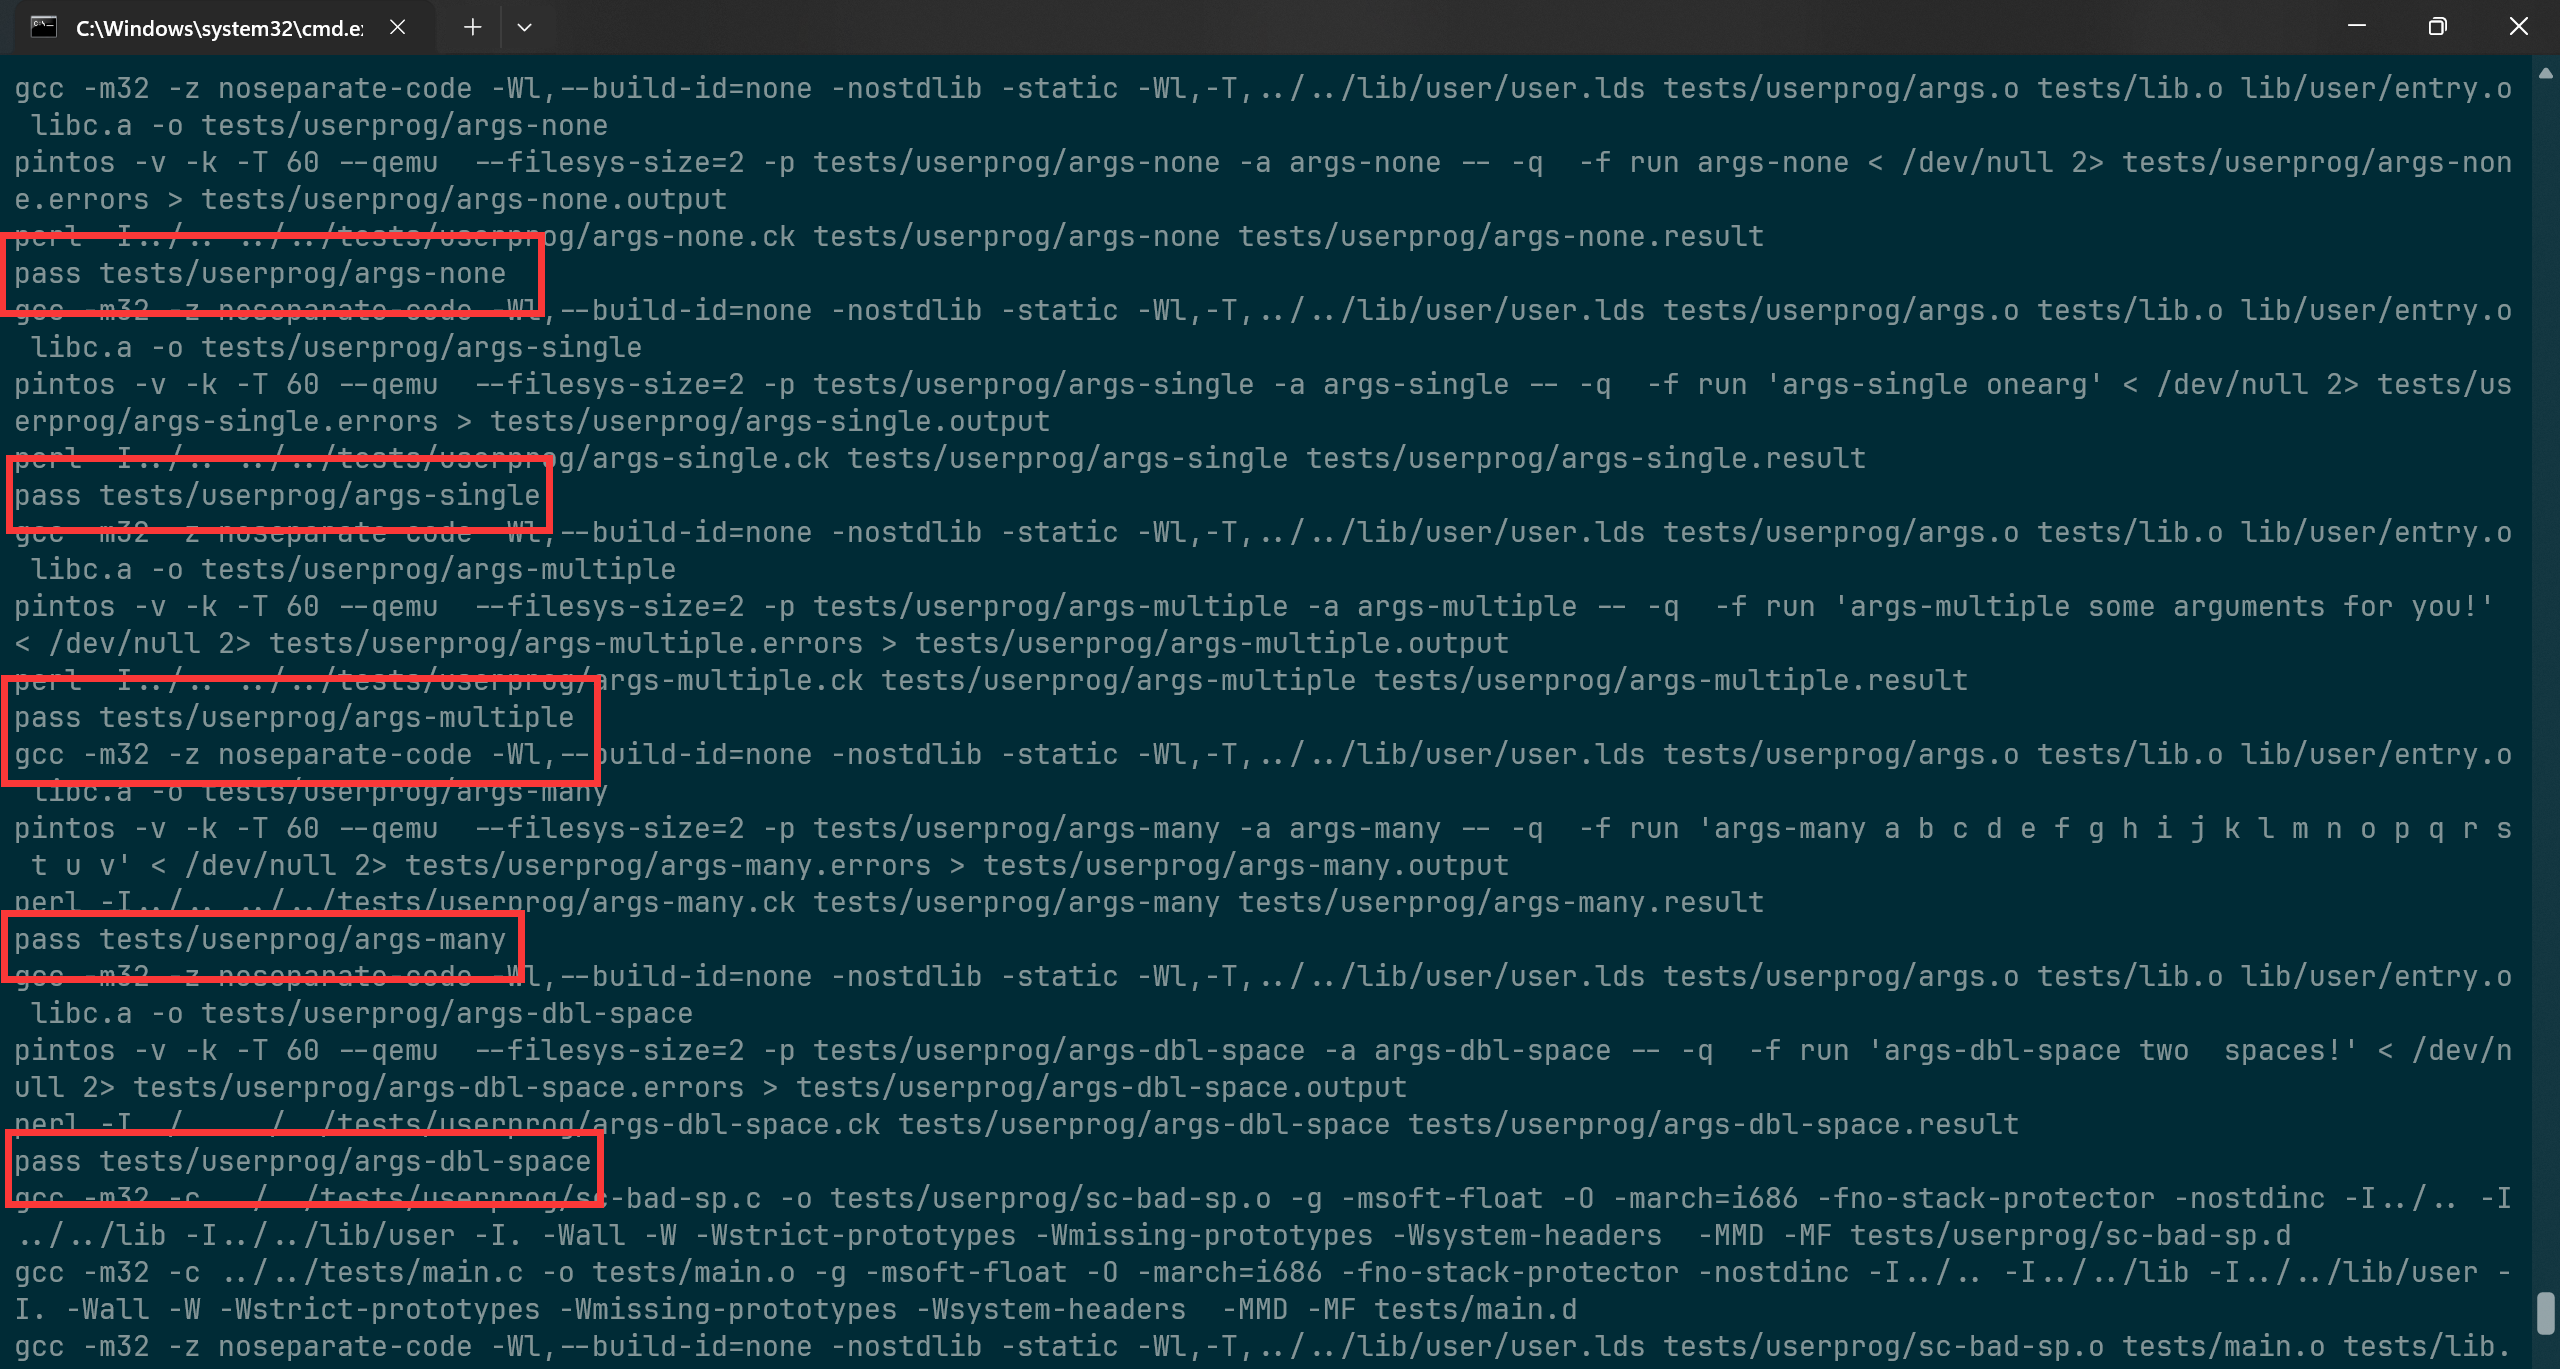
\includegraphics[width=0.9\textwidth]{img5/pass5.png}
    \caption{make check}
    \label{fig:check}
\end{figure}

等到程序最终运行完成时,可以看到 5 个与参数传递有关的测试点均已通过。

\begin{figure}[H]
    \centering
    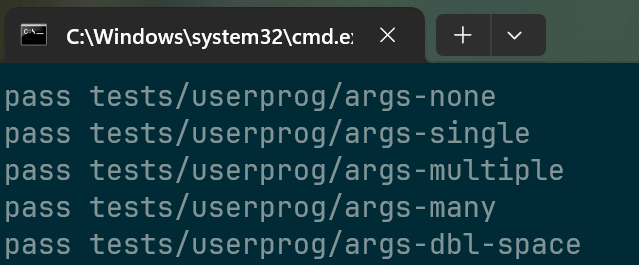
\includegraphics[width=0.45\textwidth]{img5/pass.png}
    \caption{make check}
    \label{fig:check}
\end{figure}

\section{附录}

\subsection*{参考资料}

\begin{itemize}
    \item Pintos 单一测试点代码:\href{https://pastebin.com/tFRfywvv}{\underline{https://pastebin.com/tFRfywvv}}
    \item Pintos Lab2:用户程序 User Programs(上):\href{https://blog.csdn.net/Altair_alpha/article/details/126819252}{\underline{https://blog.csdn.net/Altair\_alpha/article/details/126819252}}
    \item Pintos 指导手册:\href{https://pkuflyingpig.gitbook.io/pintos/project-description/lab2-user-programs/suggestions}{\underline{https://pkuflyingpig.gitbook.io/pintos/project-description/lab2-user-programs/suggestions}}
    \item OS实验:pintos project2:\href{https://zhuanlan.zhihu.com/p/382326973}{\underline{https://zhuanlan.zhihu.com/p/382326973}}
    \item 斯坦福大学Pintos Project1、2 指南+总结:\href{https://zhuanlan.zhihu.com/p/104497182}{\underline{https://zhuanlan.zhihu.com/p/104497182}}
\end{itemize}

\end{document}